\documentclass[12pt]{article}
\usepackage{amsmath, amssymb, amscd, amsthm, amsfonts}
\usepackage{graphicx}
\usepackage{hyperref}
\usepackage{commath}
\usepackage{subfig}
\usepackage{float}
\usepackage{listings}
\usepackage{setspace}
\usepackage[T1]{fontenc}
\oddsidemargin 0pt
\evensidemargin 0pt
\marginparwidth 40pt
\marginparsep 10pt
\topmargin -20pt
\headsep 10pt
\textheight 8.7in
\textwidth 6.65in
\linespread{2.0}

\title{ECE656 Project -- Yelp Dataset}
\author{Tiankai Jiang}
\date{\today}

\newtheorem{theorem}{Theorem}
\newtheorem{lemma}[theorem]{Lemma}
\newtheorem{conjecture}[theorem]{Conjecture}

\newcommand{\rr}{\mathbb{R}}

\newcommand{\al}{\alpha}
\DeclareMathOperator{\conv}{conv}
\DeclareMathOperator{\aff}{aff}

\makeatletter
\setlength{\@fptop}{0pt}
\makeatother
\bibliographystyle{ieeetr}

\begin{document}

\maketitle
\section{Introduction}\label{section-introduction}
Yelp dataset is a subset of Yelp's review, business and user data. The Yelp dataset used in this project is 2019 version, which contains 6,685,900 reviews, 192,609 businesses and 1,637,138 users from 10 metropolitan areas. Details of this dataset can be found \href{https://www.yelp.com/dataset/documentation/main}{here}.
\section{Data Preprocessing}\label{section-preprocessing}
\subsection{Data Preview}
We can easily check that all user\_ids in tip.json and review.json have records in user.json. But lots of user\_ids in friends are missing. And we can also check that all business\_ids in tips.json, review.json, checkin.json and photo.json are in business.json. And we can verify that the relationship between friends are mutual, that is, if A appears in B's friend list, then B will appear in A's friend list.

Also, we get the following information: all ids are 22 characters long; maximum username length is 32; maximum business name length is 64; maximum review length is 5000 and maximum tip length is 500. 

The most complex part is the attributes and categories in business information. There are 1300 different categories and 39 different attributes for business. In those attributes, 32 of them have a single value, e.g. "True", "False", "None". The rest of them contain nested structure, which means their value is again, a dictionary. E.g. attribute "BestNights" refers to a dictionary, with each day in a week as a key and "True", "False" as value. Some attributes and categories have a null value, or the field "attribute"/"category" itself is null.

Furthermore, some fields in business.json contain a leading letter "u", e.g. u"True", which means a unicode string. We should remove letter "u" since "True" and u"True" have the same meaning.
\subsection{Data Cleaning}
Remove all user\_ids that appear only in friends list but not in "user\_id" column from user.json. And remove all character "u" before texts from business.json.
\section{Relational Database}\label{section-database}
\subsection{Design}
The ER Diagram of the database is shown as follows. The primary key of a table is in bold and the foreign keys are highlighted in light blue.
\begin{figure}[H]
\begin{center}
    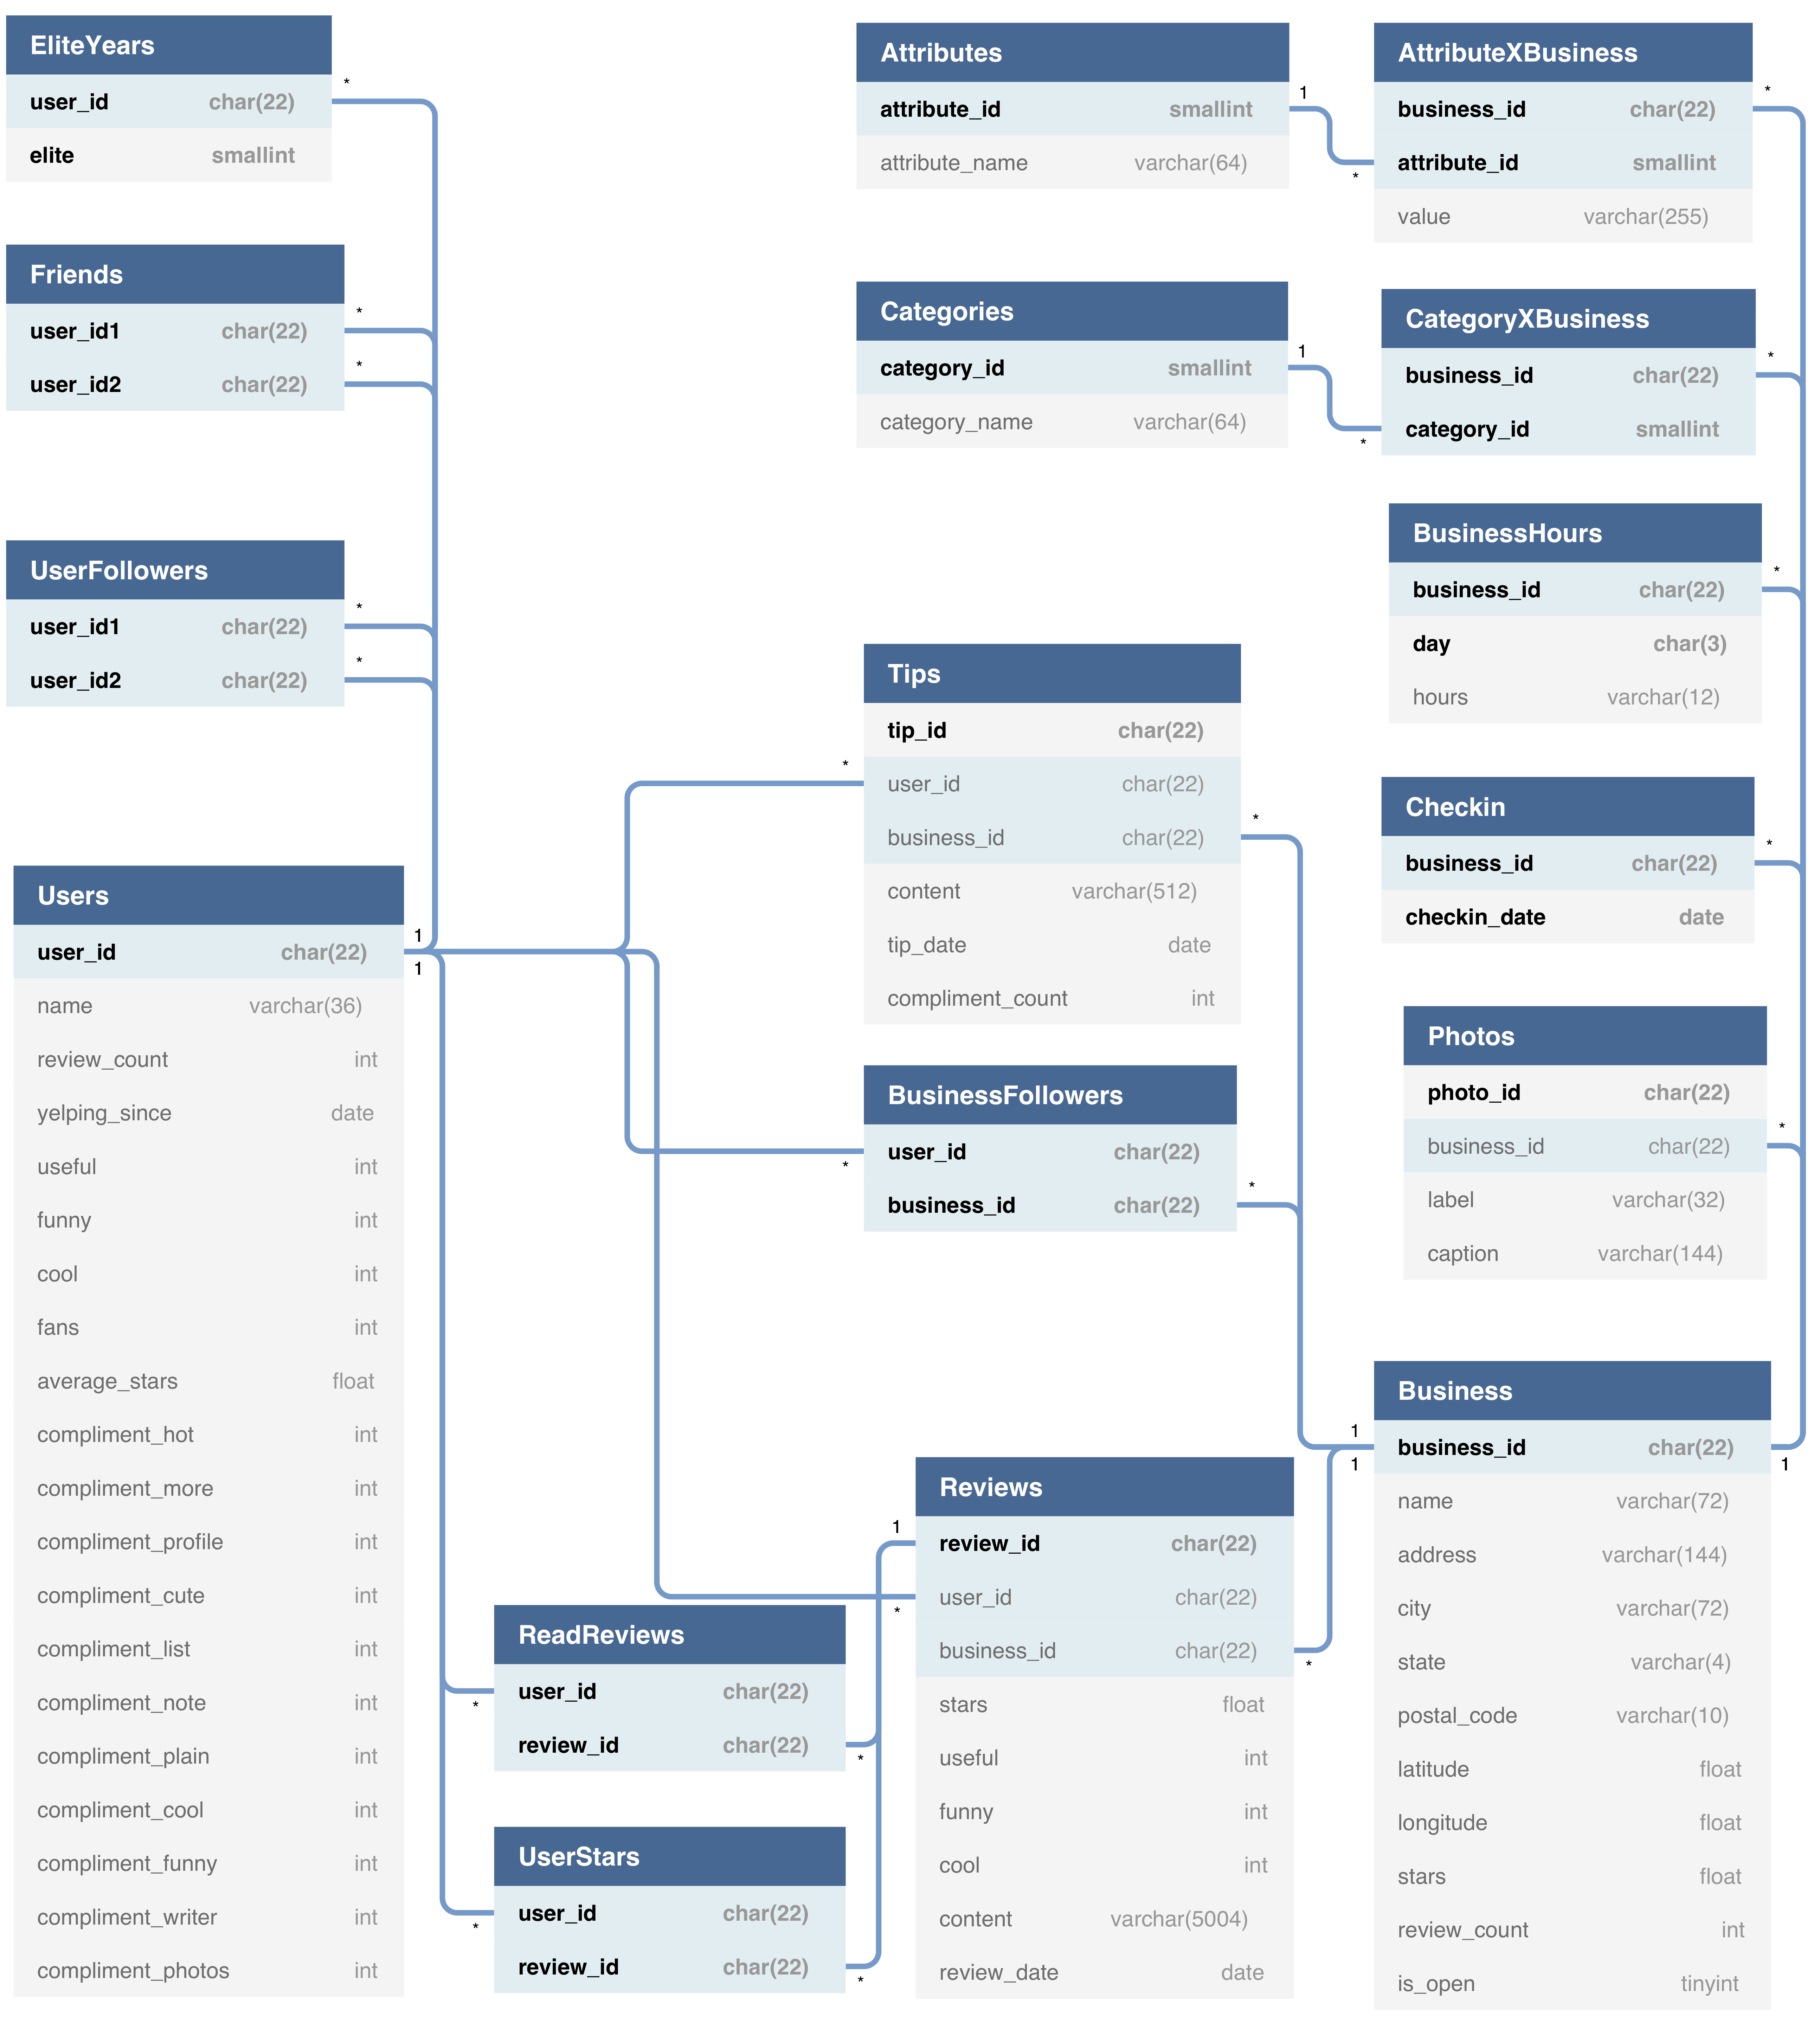
\includegraphics[width=1.0\textwidth]{ER_Diagram.png}
\end{center}
\end{figure}
Five main tables in the diagram are {\it Users}, {\it Business}, {\it Reviews}, {\it Photos} and {\it Tips}. Each row of table {\it EliteYears} stores a user\_id and a year number. Table {\it Friends} stores pairs of users. Table {\it Attributes} and table {\it Categories} store ids and names of attributes/categories and connect with {\it Business} through junction table {\it AttributeXBusiness} and {\it CategoryXBusiness}. All values of attributes are stored as string no matter the value is "True"/"False" or a dictionary since they are not our focus in the following analysis, and spliting all of them apart will complicate the design. Table {\it BusinessHours} stores the hours of a business, each day per row, and days are expressed in three characters, from "Mon" to "Sun". Table {\it UserFollowers, BusinessFollowers, ReadReviews} and {\it UserStars} are used for the api and they are not part of the original data.
\subsection{Dumping Data}
Extract all data for tables from json files into individual files, at the same time adding required missing fields such as tip\_id, and then write those files to database. Files should be read as raw string since there are lots of special characters in them.
\section{Server and Client}\label{section-api}
Flask is used as the web framework.
\subsection{API}
16 operations are supported in the API. The status in the responsed json will be 0 if the operation succeeded, otherwise 1, with the error message in message field.

\subsubsection{Login}
\textbf{Description:}\\
Login as an existing user.\\
\textbf{Method:}\\
POST\\
\textbf{API call:}\\ 
http://127.0.0.1:5000/yelp/login\\
\textbf{Parameters:}\\
user\_id: your user\_id\\
\textbf{API Response:}

\begin{singlespacing}
\begin{lstlisting}
{
 "message": "___DPmKJsBF2X6ZKgAeGqg",
 "status": 0
}
\end{lstlisting}
\end{singlespacing}

\subsubsection{Register}
\textbf{Description:}\\
Register a new user account.\\
\textbf{Method:}\\
POST\\
\textbf{API call:}\\
http://127.0.0.1:5000/yelp/newuser\\
\textbf{Parameters:}\\
username: username for the new account\\
\textbf{API Response:}

\begin{singlespacing}
\begin{lstlisting}
{
 "message": "qkVPN3ZeXKxD-2y_bewUEk",
 "status": 0
}
\end{lstlisting}
\end{singlespacing}

\subsubsection{Star/Unstar}
\textbf{Description:}\\
Star/Unstar a review.\\
\textbf{Method:}\\
POST\\
\textbf{API call:}\\
http://127.0.0.1:5000/yelp/star\\
\textbf{Parameters:}\\
user\_id: your user\_id\\
review\_id: an existing review\_id\\
\textbf{API Response:}

\begin{singlespacing}
\begin{lstlisting}
{
 "message": "Starred",
 "status": 0
}
\end{lstlisting}
\end{singlespacing}

\subsubsection{Get all Starred Reviews}
\textbf{Description:}\\
Retrieve all reviews you have starred.\\
\textbf{Method:}\\
GET\\
\textbf{API call:}\\
http://127.0.0.1:5000/yelp/stars?u=\{user\_id\}\\
\textbf{Parameters:}\\
user\_id: your user\_id\\
\textbf{API Response:}

\begin{singlespacing}
\begin{lstlisting}
{
 "message": [
  {
   "business": "Pure Indian Cuisine",
   "reviewID": "___-Bw8LtQgezPiN9xJWaQ",
   "reviewer": "David",
   "snippet": "Don't know how I missed this place after so m...",
   "stars": 6.0
  }
 ],
 "status": 0
}
\end{lstlisting}
\end{singlespacing}

\subsubsection{New Review}
\textbf{Description:}\\
Post a new review\\
\textbf{Method:}\\
POST\\
\textbf{API call:}\\
http://127.0.0.1:5000/yelp/newpost\\
\textbf{Parameters:}\\
user\_id: your user\_id\\
business\_id: the business\_id of the business you want to comment on\\
content: review content\\
\textbf{API Response:}

\begin{singlespacing}
\begin{lstlisting}
{
 "message": "NnoOqAoBXsoqOWJVsTakBK",
 "status": 0
}
\end{lstlisting}
\end{singlespacing}

\subsubsection{Follow/Unfollow a User}
\textbf{Description:}\\
Follow/Unfollow a user.\\
\textbf{Method:}\\
POST\\
\textbf{API call:}\\
http://127.0.0.1:5000/yelp/followu\\
\textbf{Parameters:}\\
user\_id1: your user\_id\\
user\_id2: user\_id of the person you want to follow\\
\textbf{API Response:}

\begin{singlespacing}
\begin{lstlisting}
{
 "message": "Unfollowed",
 "status": 0
}
\end{lstlisting}
\end{singlespacing}

\subsubsection{Follow/Unfollow a Business}
\textbf{Description:}\\
Follow/Unfollow a business.\\
\textbf{Method:}\\
POST\\
\textbf{API call:}\\
http://127.0.0.1:5000/yelp/followb\\
\textbf{Parameters:}\\
user\_id: your user\_id\\
business\_id: business\_id of the business you want to follow\\
\textbf{API Response:}

\begin{singlespacing}
\begin{lstlisting}
{
 "message": "Followed",
 "status": 0
}
\end{lstlisting}
\end{singlespacing}

\subsubsection{Get All New Reviews1}
\textbf{Description:}\\
Get all new reviews by people you have followed.\\
\textbf{Method:}\\
GET\\
\textbf{API call:}\\ 
http://127.0.0.1:5000/yelp/uposts?u=\{user\_id\}\&l=\{number\}\\
\textbf{Parameters:}\\
user\_id: your user\_id\\
number(optional): number of posts to get, or empty to retrieve all\\
\textbf{API Response:}

\begin{singlespacing}
\begin{lstlisting}
{
 "message": [
  {
   "business_name": "Brake Masters",
   "review_id": "c4B3NGDZbQnRgbe4fw6qGw",
   "content": "review content 1",
   "reviewer": "Charlotte",
   "review_date": "Thu, 22 May 2014 20:20:14 GMT"
  },
  {
   "business_name": "The Watershed",
   "review_id": "GGg4KdkyvbdHwdwsC46l7g",
   "content": "review content 2",
   "reviewer": "Charlotte",
   "review_date": "Mon, 03 Aug 2015 22:26:54 GMT"
  }
 ],
 "status": 0
}
\end{lstlisting}
\end{singlespacing}

\subsubsection{Get All New Reviews2}
\textbf{Description:}\\
Get all new reviews of the business you have followed.\\
\textbf{Method:}\\
GET\\
\textbf{API call:}\\ 
http://127.0.0.1:5000/yelp/bposts?u=\{user\_id\}\&l=\{number\}\\
\textbf{Parameters:}\\
user\_id: your user\_id\\
number(optional): number of posts to get, or empty to retrieve all\\
\textbf{API Response:}

\begin{singlespacing}
\begin{lstlisting}
{
 "message": [
  {
   "business_name": "Brake Masters",
   "review_id": "c4B3NGDZbQnRgbe4fw6qGw",
   "content": "review content 1",
   "reviewer": "Charlotte",
   "review_date": "Thu, 22 May 2014 20:20:14 GMT"
  },
  {
   "business_name": "The Watershed",
   "review_id": "GGg4KdkyvbdHwdwsC46l7g",
   "content": "review content 2",
   "reviewer": "Charlotte",
   "review_date": "Mon, 03 Aug 2015 22:26:54 GMT"
  }
 ],
 "status": 0
}
\end{lstlisting}
\end{singlespacing}

\subsubsection{My Reviews}
\textbf{Description:}\\
Get all your posted reviews\\
\textbf{Method:}\\
GET\\
\textbf{API call:}\\ 
http://127.0.0.1:5000/yelp/mposts?u=\{user\_id\}\\
\textbf{Parameters:}\\
user\_id: your user\_id\\
\textbf{API Response:}

\begin{singlespacing}
\begin{lstlisting}
{
 "message": [
  {
   "business_name": "The Range 702",
   "content": "review content",
   "cool": 0,
   "funny": 0,
   "review_date": "Wed, 05 Aug 2015 07:20:13 GMT",
   "review_id": "Ph4MAecNE-sTQK1Fnf6E7Q",
   "stars": 5.0,
   "useful": 0
  }
 ],
 "status": 0
}
\end{lstlisting}
\end{singlespacing}

\subsubsection{Followed Users}
\textbf{Description:}\\
Get all your followed users.\\
\textbf{Method:}\\
GET\\
\textbf{API call:}\\ 
http://127.0.0.1:5000/yelp/followulist?u=\{user\_id\}\\
\textbf{Parameters:}\\
user\_id: your user\_id\\
\textbf{API Response:}

\begin{singlespacing}
\begin{lstlisting}
{
 "message": [
  {
   "name": "Charlotte",
   "user_id": "___DPmKJsBF2X6ZKgAeGqg"
  }
 ],
 "status": 0
}
\end{lstlisting}
\end{singlespacing}

\subsubsection{Followed Business}
\textbf{Description:}\\
Get all your followed business.\\
\textbf{Method:}\\
GET\\
\textbf{API call:}\\ 
http://127.0.0.1:5000/yelp/followblist?u=\{user\_id\}\\
\textbf{Parameters:}\\
user\_id: your user\_id\\
\textbf{API Response:}

\begin{singlespacing}
\begin{lstlisting}
{
 "message": [
  {
   "business_id": "__1uG7MLxWGFIv2fCGPiQQ",
   "name": "SpinalWorks Chiropractic",
   "stars": 5.0
  },
  {
   "business_id": "9Q1ZtzTPFWG4fJiFSko5Xg",
   "name": "Cantina Laredo",
   "stars": 3.5
  }
 ],
 "status": 0
}
\end{lstlisting}
\end{singlespacing}

\subsubsection{Delete Review}
\textbf{Description:}\\
Remove your posted review.\\
\textbf{Method:}\\
POST\\
\textbf{API call:}\\ 
http://127.0.0.1:5000/yelp/dpost?u=\{user\_id\}\&r=\{review\_id\}\\
\textbf{Parameters:}\\
user\_id: your user\_id\\
review\_id: the id of the review you want to delete\\
\textbf{API Response:}

\begin{singlespacing}
\begin{lstlisting}
{
 "message": "Success",
 "status": 0
}
\end{lstlisting}
\end{singlespacing}

\subsubsection{Change username}
\textbf{Description:}\\
Change your account username.\\
\textbf{Method:}\\
POST\\
\textbf{API call:}\\ 
http://127.0.0.1:5000/yelp/cn\\
\textbf{Parameters:}\\
user\_id: your user\_id\\
username: the username you want to set\\
\textbf{API Response:}

\begin{singlespacing}
\begin{lstlisting}
{
 "message": "Success",
 "status": 0
}
\end{lstlisting}
\end{singlespacing}

\subsubsection{Who Am I}
\textbf{Description:}\\
Display your account information.\\
\textbf{Method:}\\
GET\\
\textbf{API call:}\\ 
http://127.0.0.1:5000/yelp/whoami?u=\{user\_id\}\\
\textbf{Parameters:}\\
user\_id: your user\_id\\
\textbf{API Response:}

\begin{singlespacing}
\begin{lstlisting}
{
 "message": [
  {
   "cool": 0,
   "fans": 0,
   "funny": 0,
   "name": "Mike",
   "reviews": 5,
   "stars": 5.0,
   "useful": 1,
   "user_id": "___QCazm0YrHLd3uNUPYMA",
   "yelping_since": "Thu, 31 Jul 2014 21:53:24 GMT"
  }
 ],
 "status": 0
}
\end{lstlisting}
\end{singlespacing}

\subsubsection{Reset}
\textbf{Description:}\\
Reset read history so that you can see the read reviews again.\\
\textbf{Method:}\\
POST\\
\textbf{API call:}\\ 
http://127.0.0.1:5000/yelp/reset\\
\textbf{Parameters:}\\
user\_id: your user\_id\\
\textbf{API Response:}

\begin{singlespacing}
\begin{lstlisting}
{
 "message": "Success",
 "status": 0
}
\end{lstlisting}
\end{singlespacing}

\subsection{Client}
Please check the uploaded video.

\section{Data Mining}\label{section-datamining}
\subsection{Data Visualization}
\subsubsection{Top 20 Categories in Business}
\begin{figure}[H]
\begin{center}
    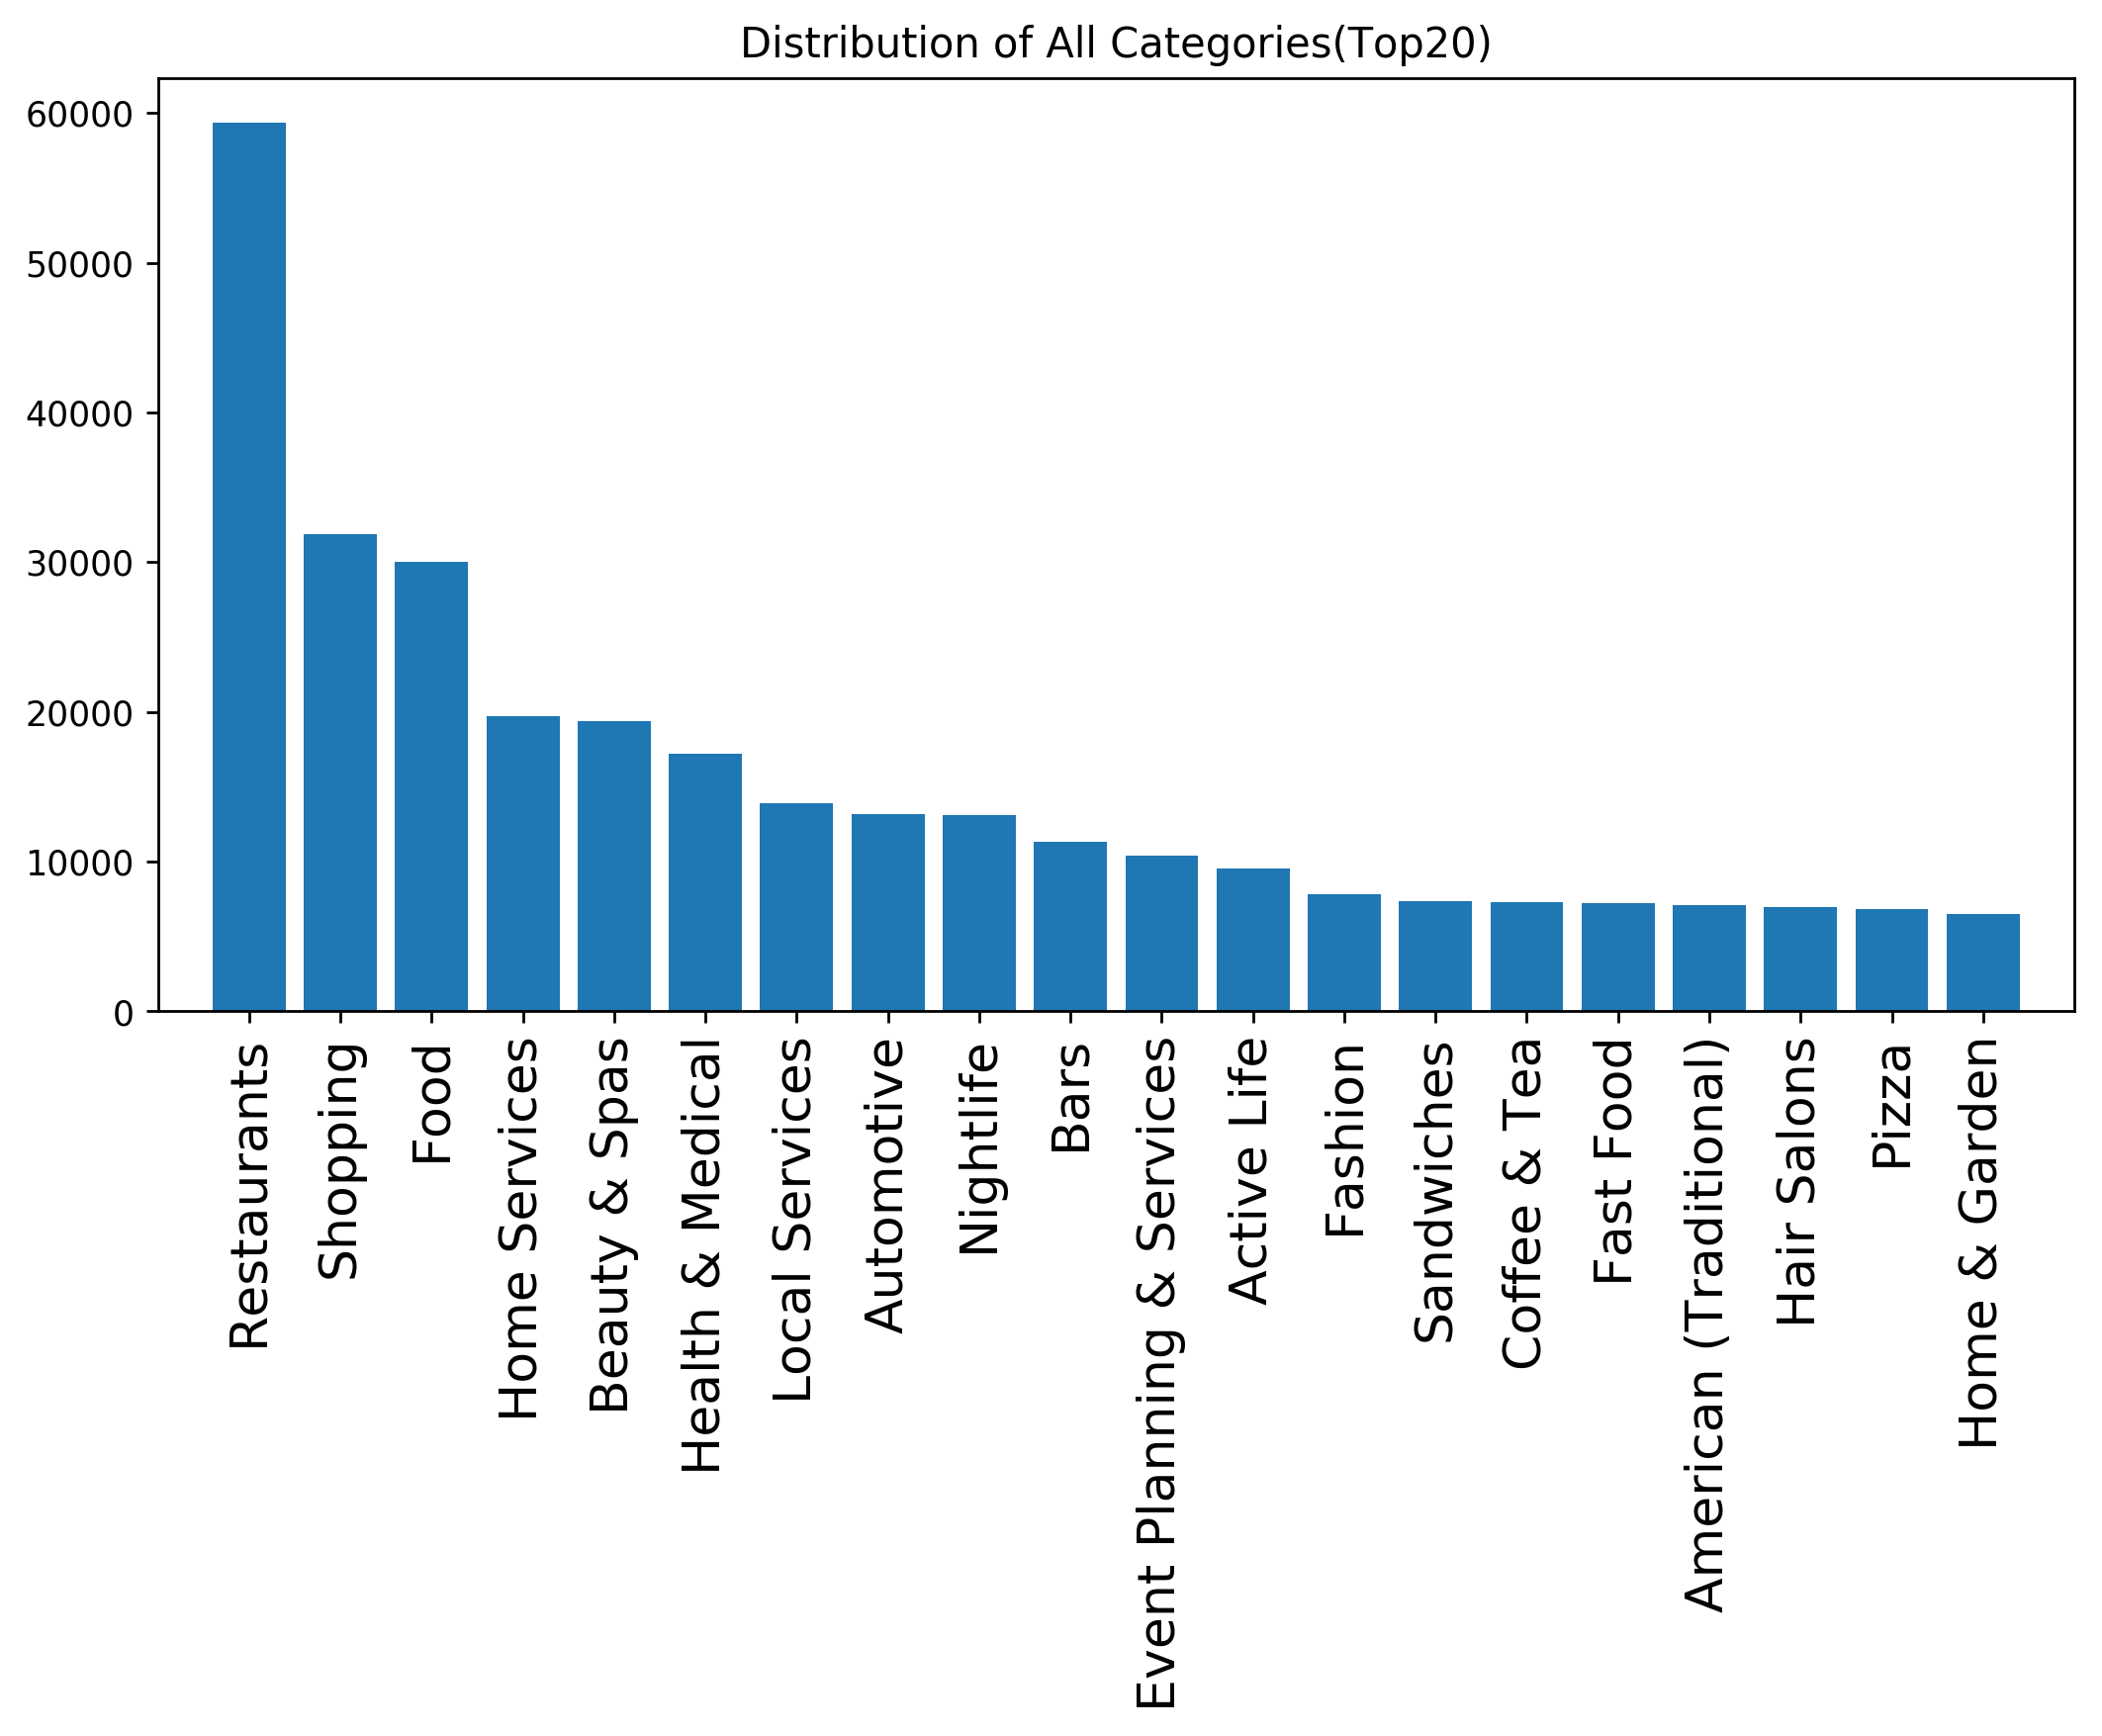
\includegraphics[width=1.0\textwidth]{../05_dataMining/distributionAllCategories.png}
\end{center}
\end{figure}
The most common category in the dataset is restaurant. There are about 60 thousand restaurants, followed by shopping, home services and beauty\&Spas.

\subsubsection{Top 50 Categories in Restaurants}
\begin{figure}[H]
\begin{center}
    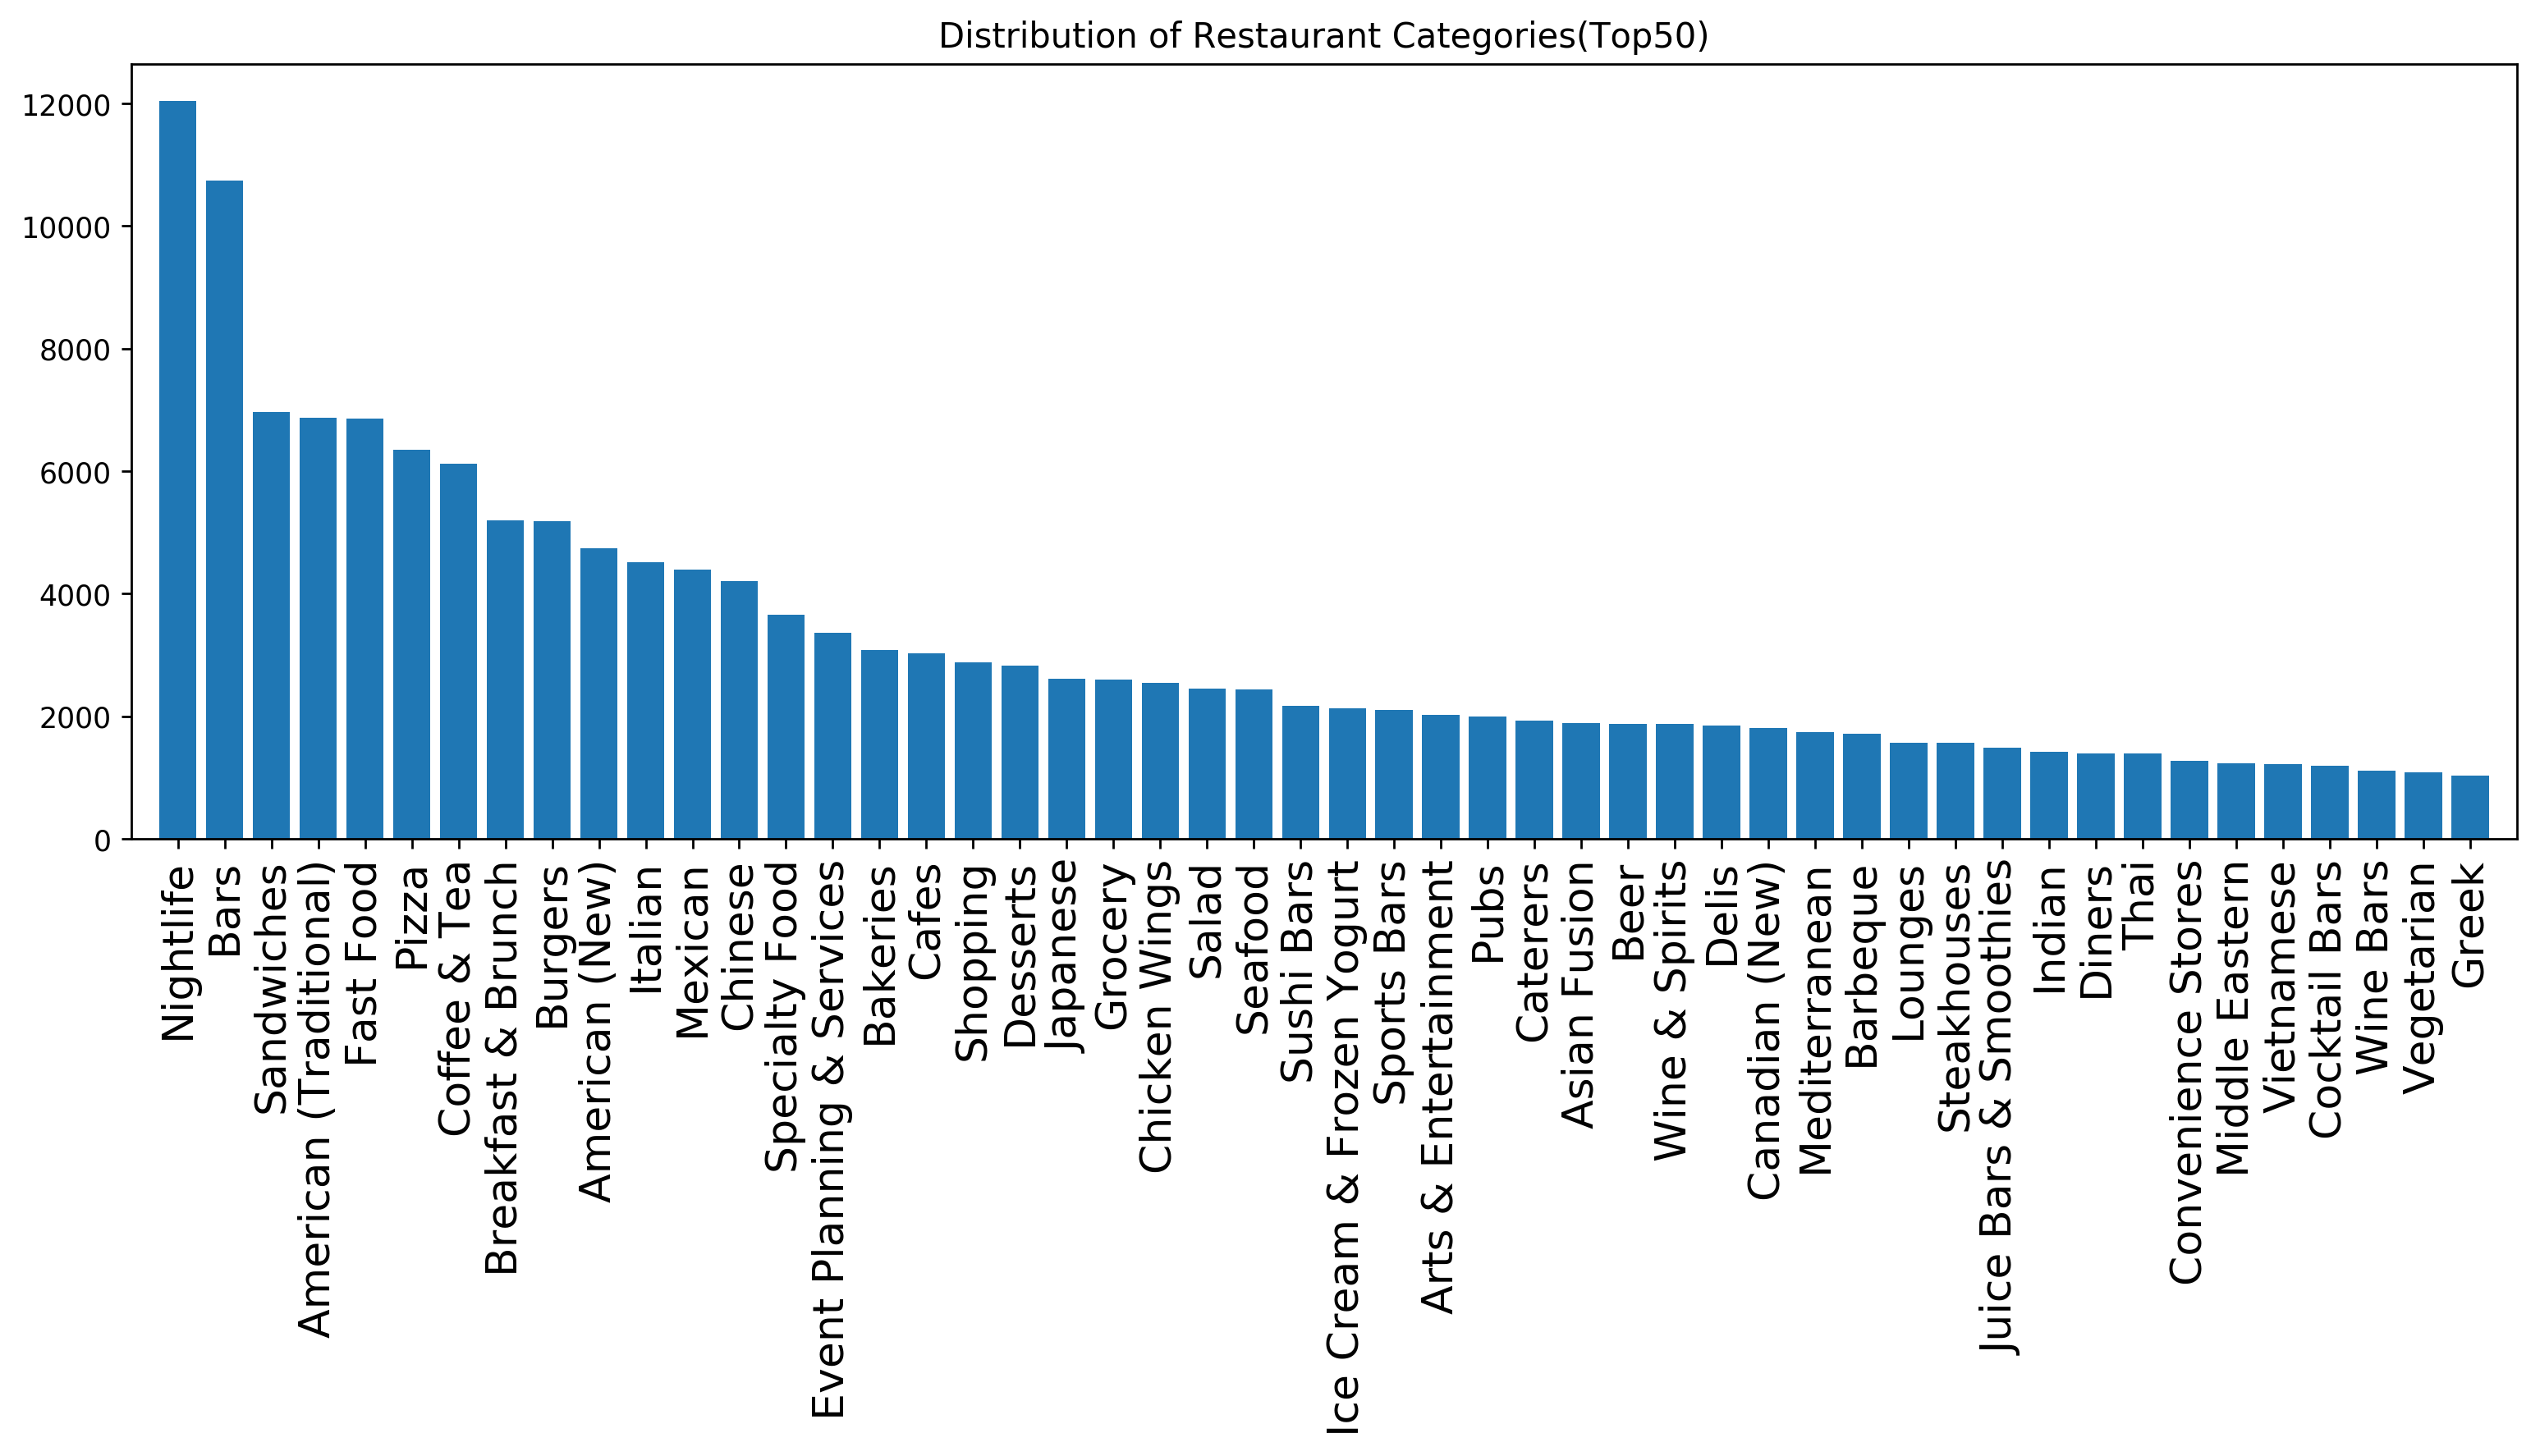
\includegraphics[width=1.0\textwidth]{../05_dataMining/distributionRestaurants.png}
\end{center}
\end{figure}
Since basically every restaurant has attribute {\it Restaurant} and {\it Food}, we plot the graph starting from the third most attribute. Generally, bars and all kinds of fast food are the most common categories.

\subsubsection{Distribution of Business Score}
\begin{figure}[H]
\captionsetup[subfigure]{labelformat=empty}
\centering
\subfloat[]{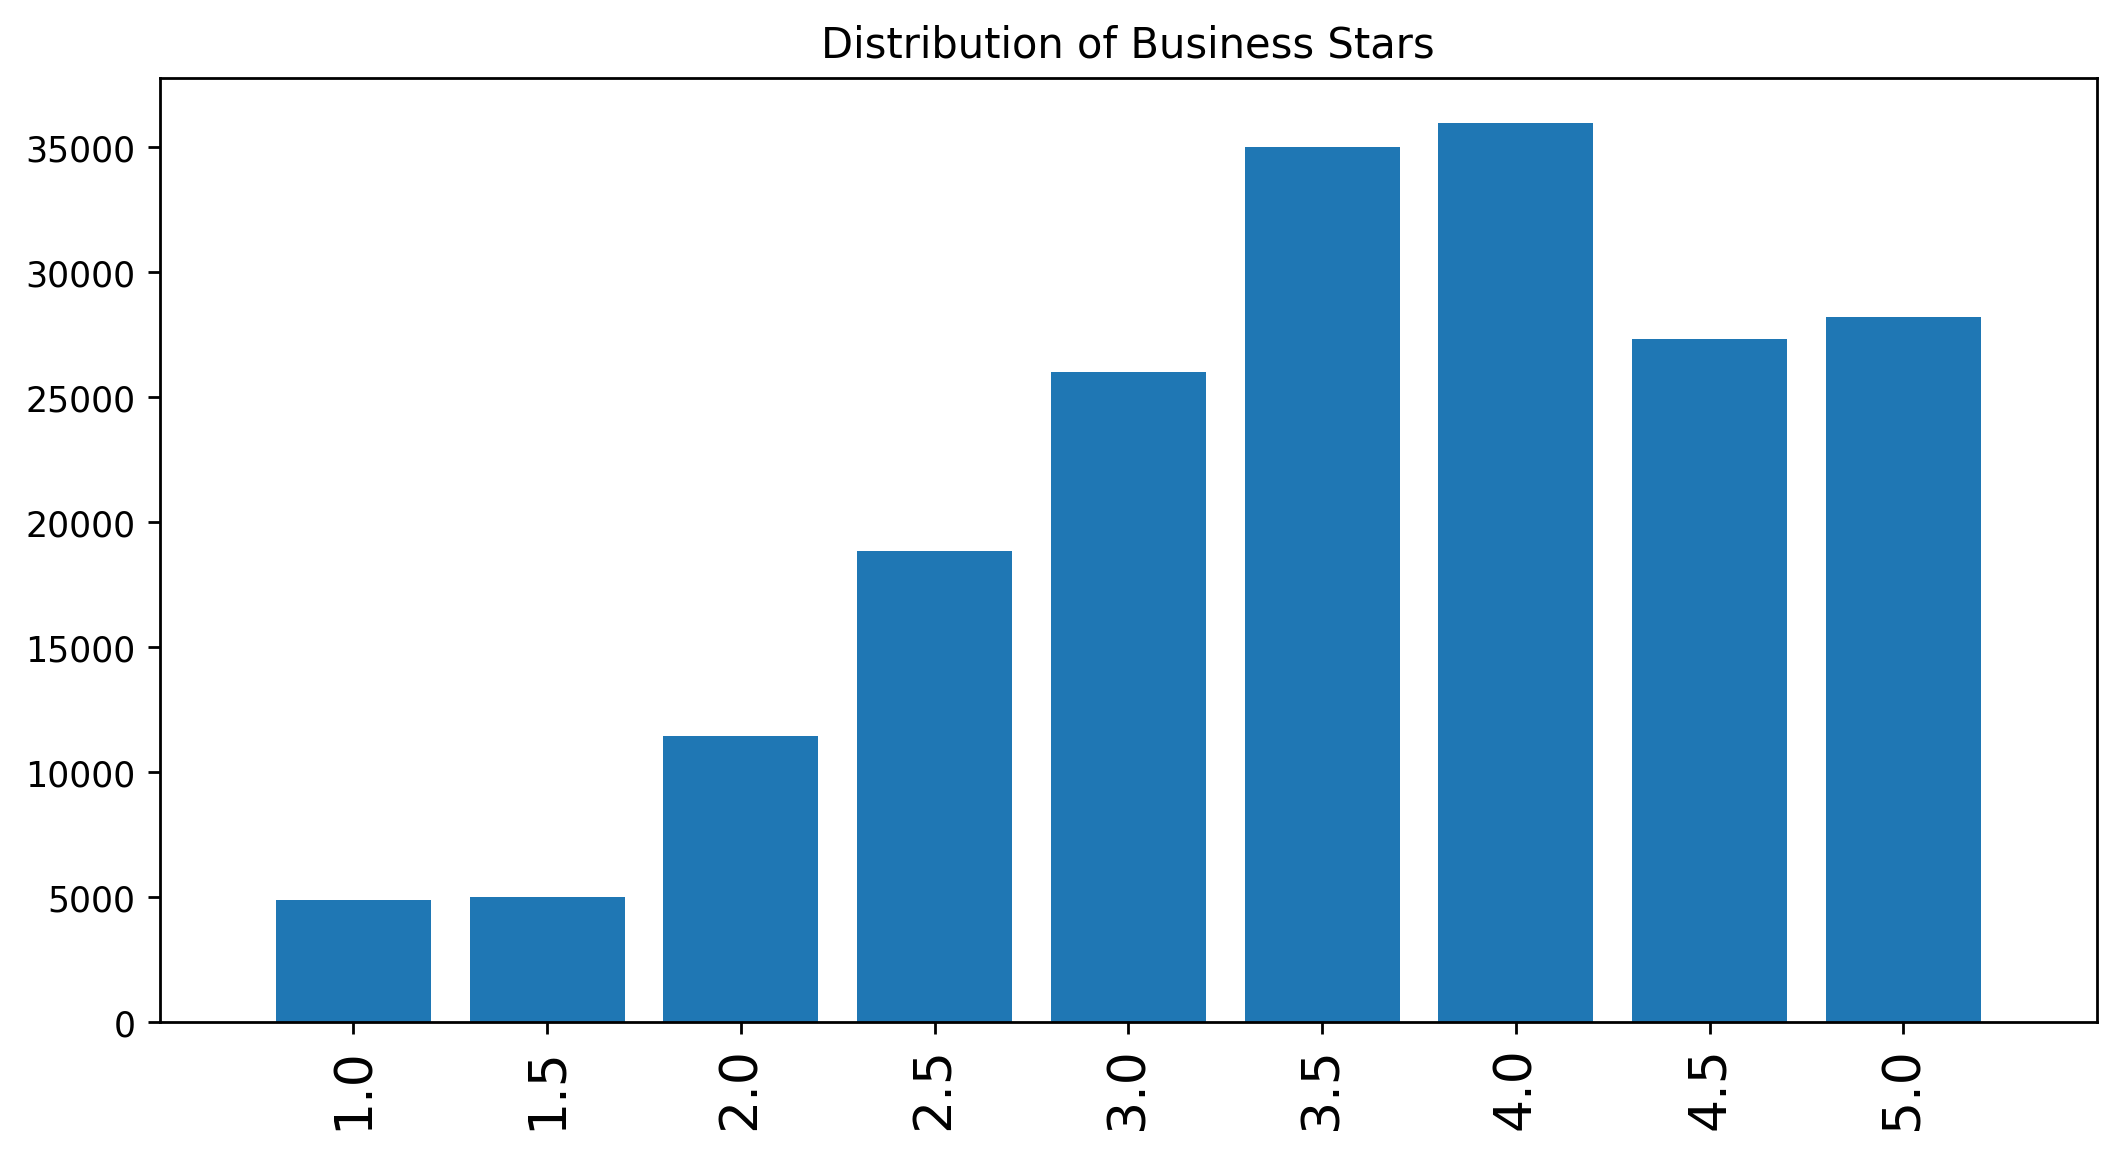
\includegraphics[width=0.6\textwidth]{../05_dataMining/distributionBusinessStars.png}}
\subfloat[] {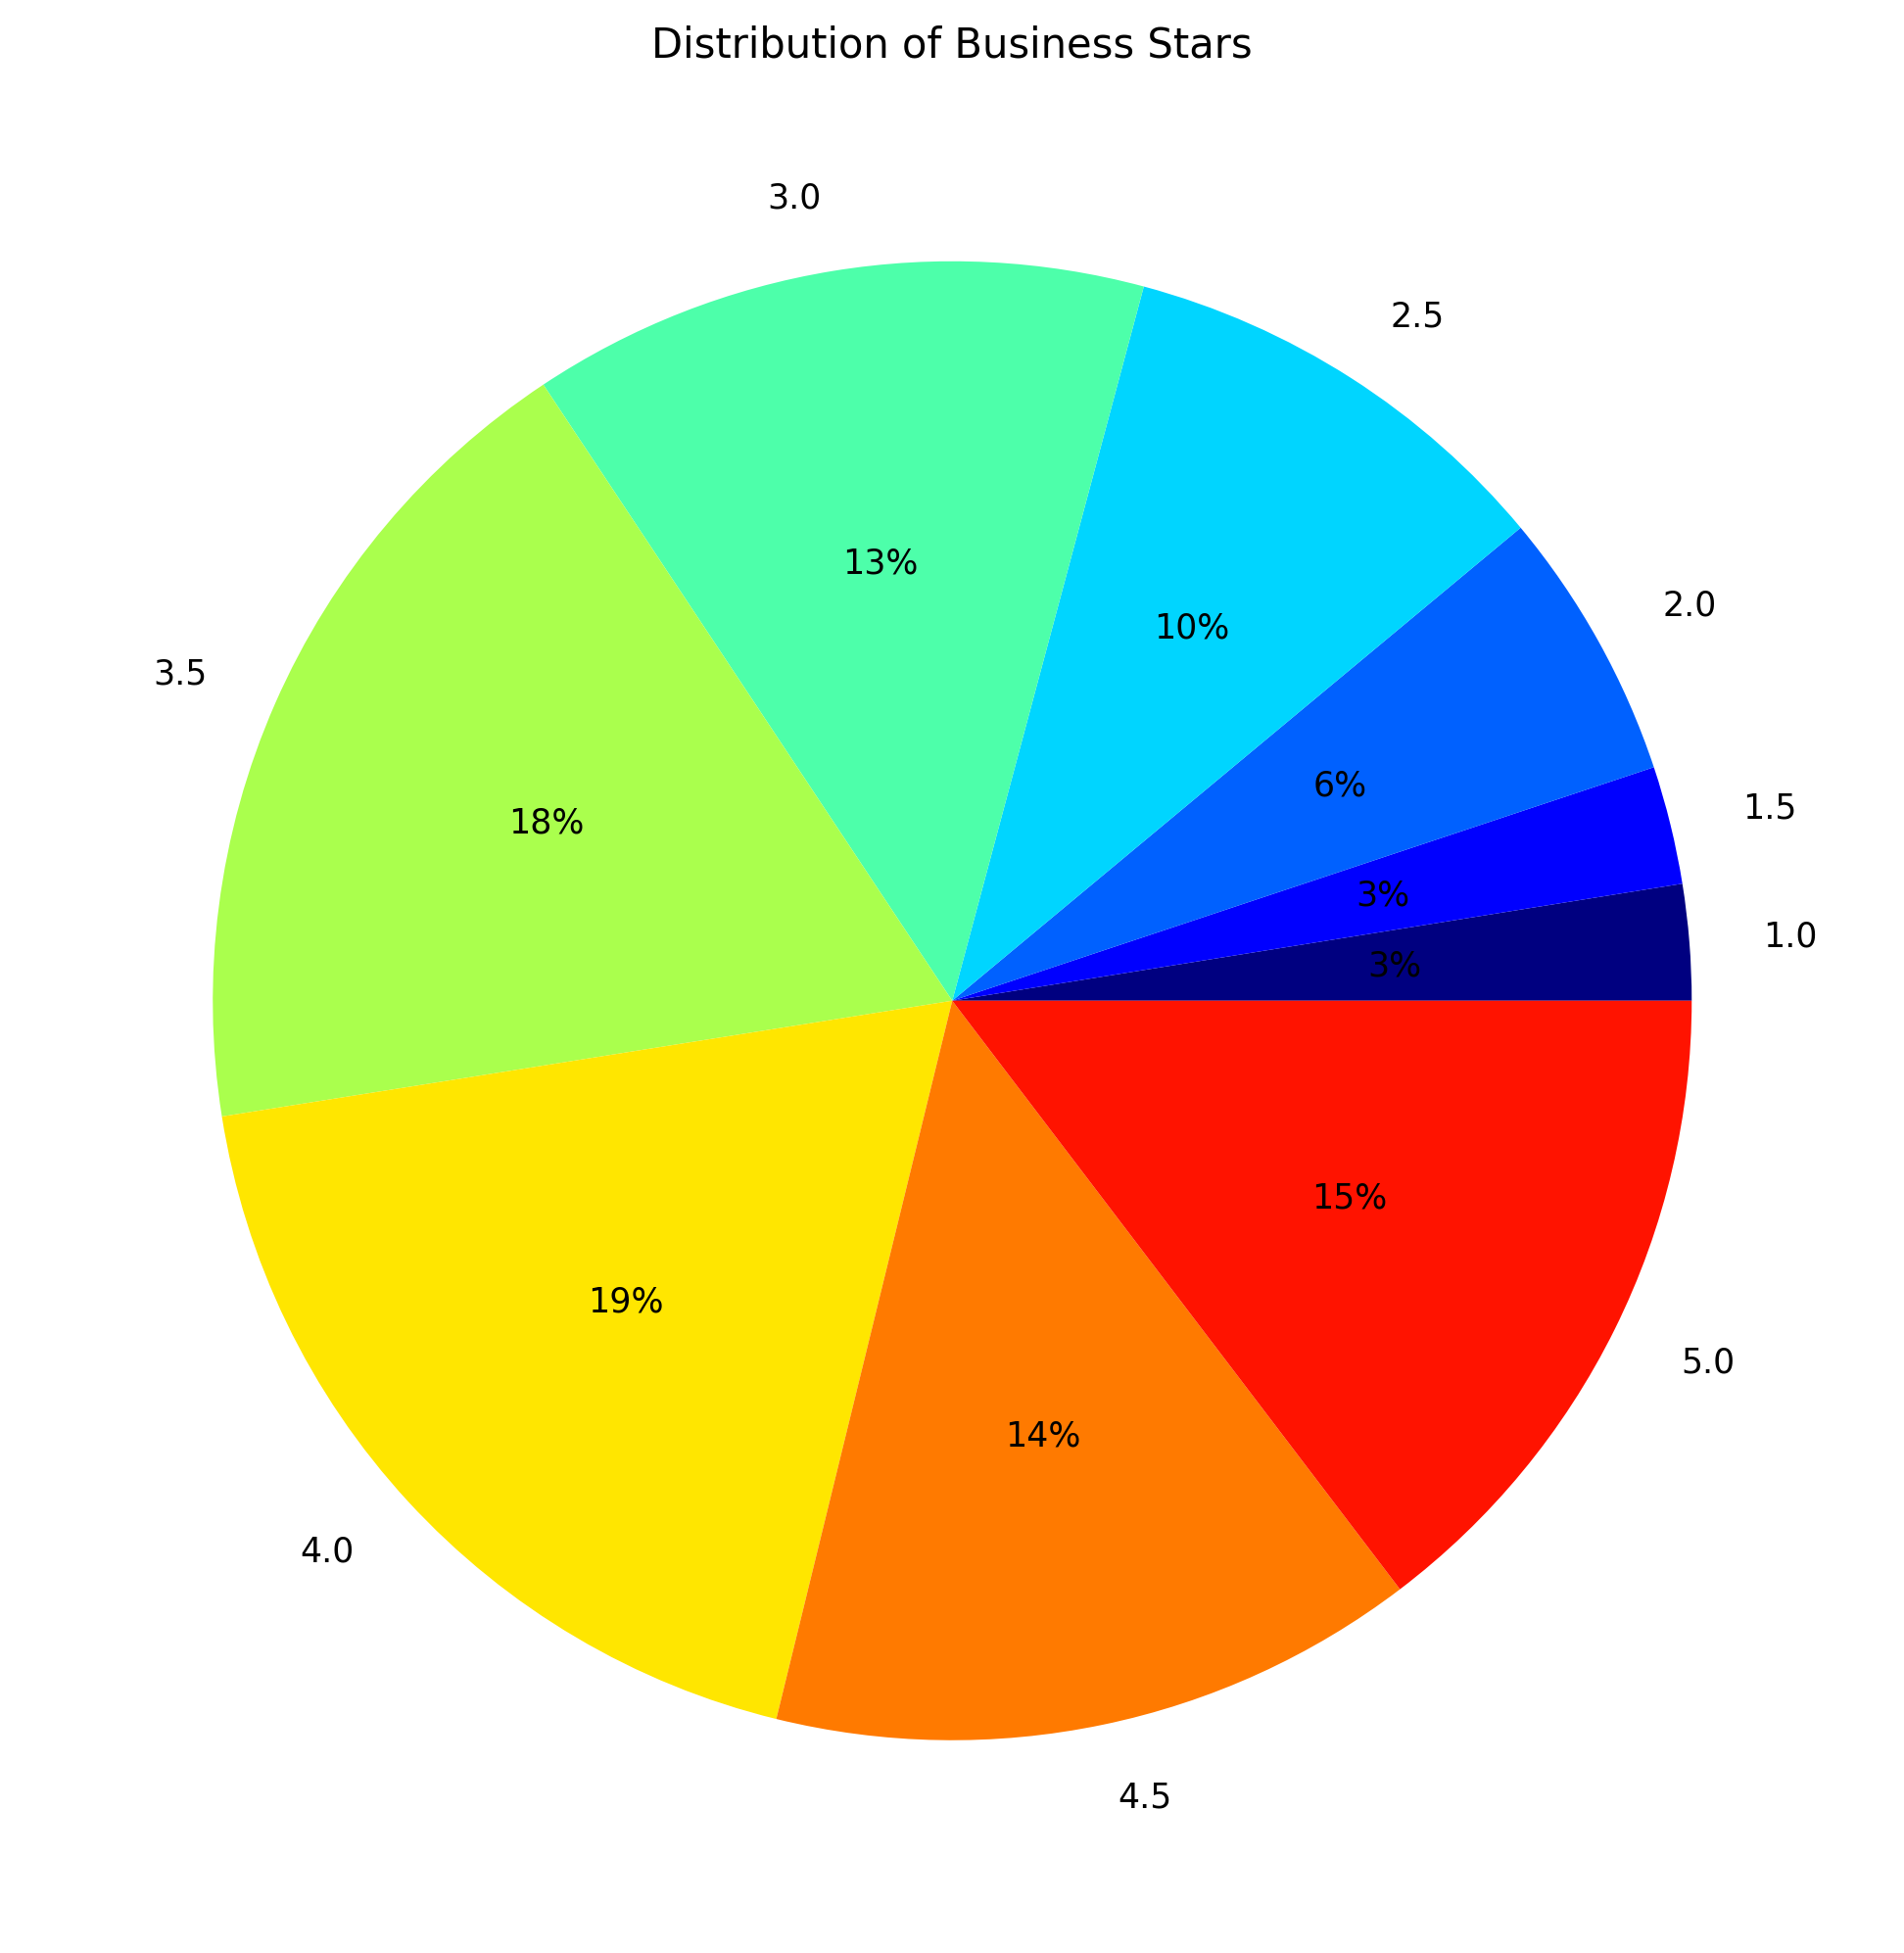
\includegraphics[width=0.4\textwidth]{../05_dataMining/distributionBusinessStarsPie.png}}
\end{figure}
About 80 percent of the business has a score greater or equal than 3.0.

\subsubsection{Geographical Distribution of the Business}
\begin{figure}[H]
\begin{center}
    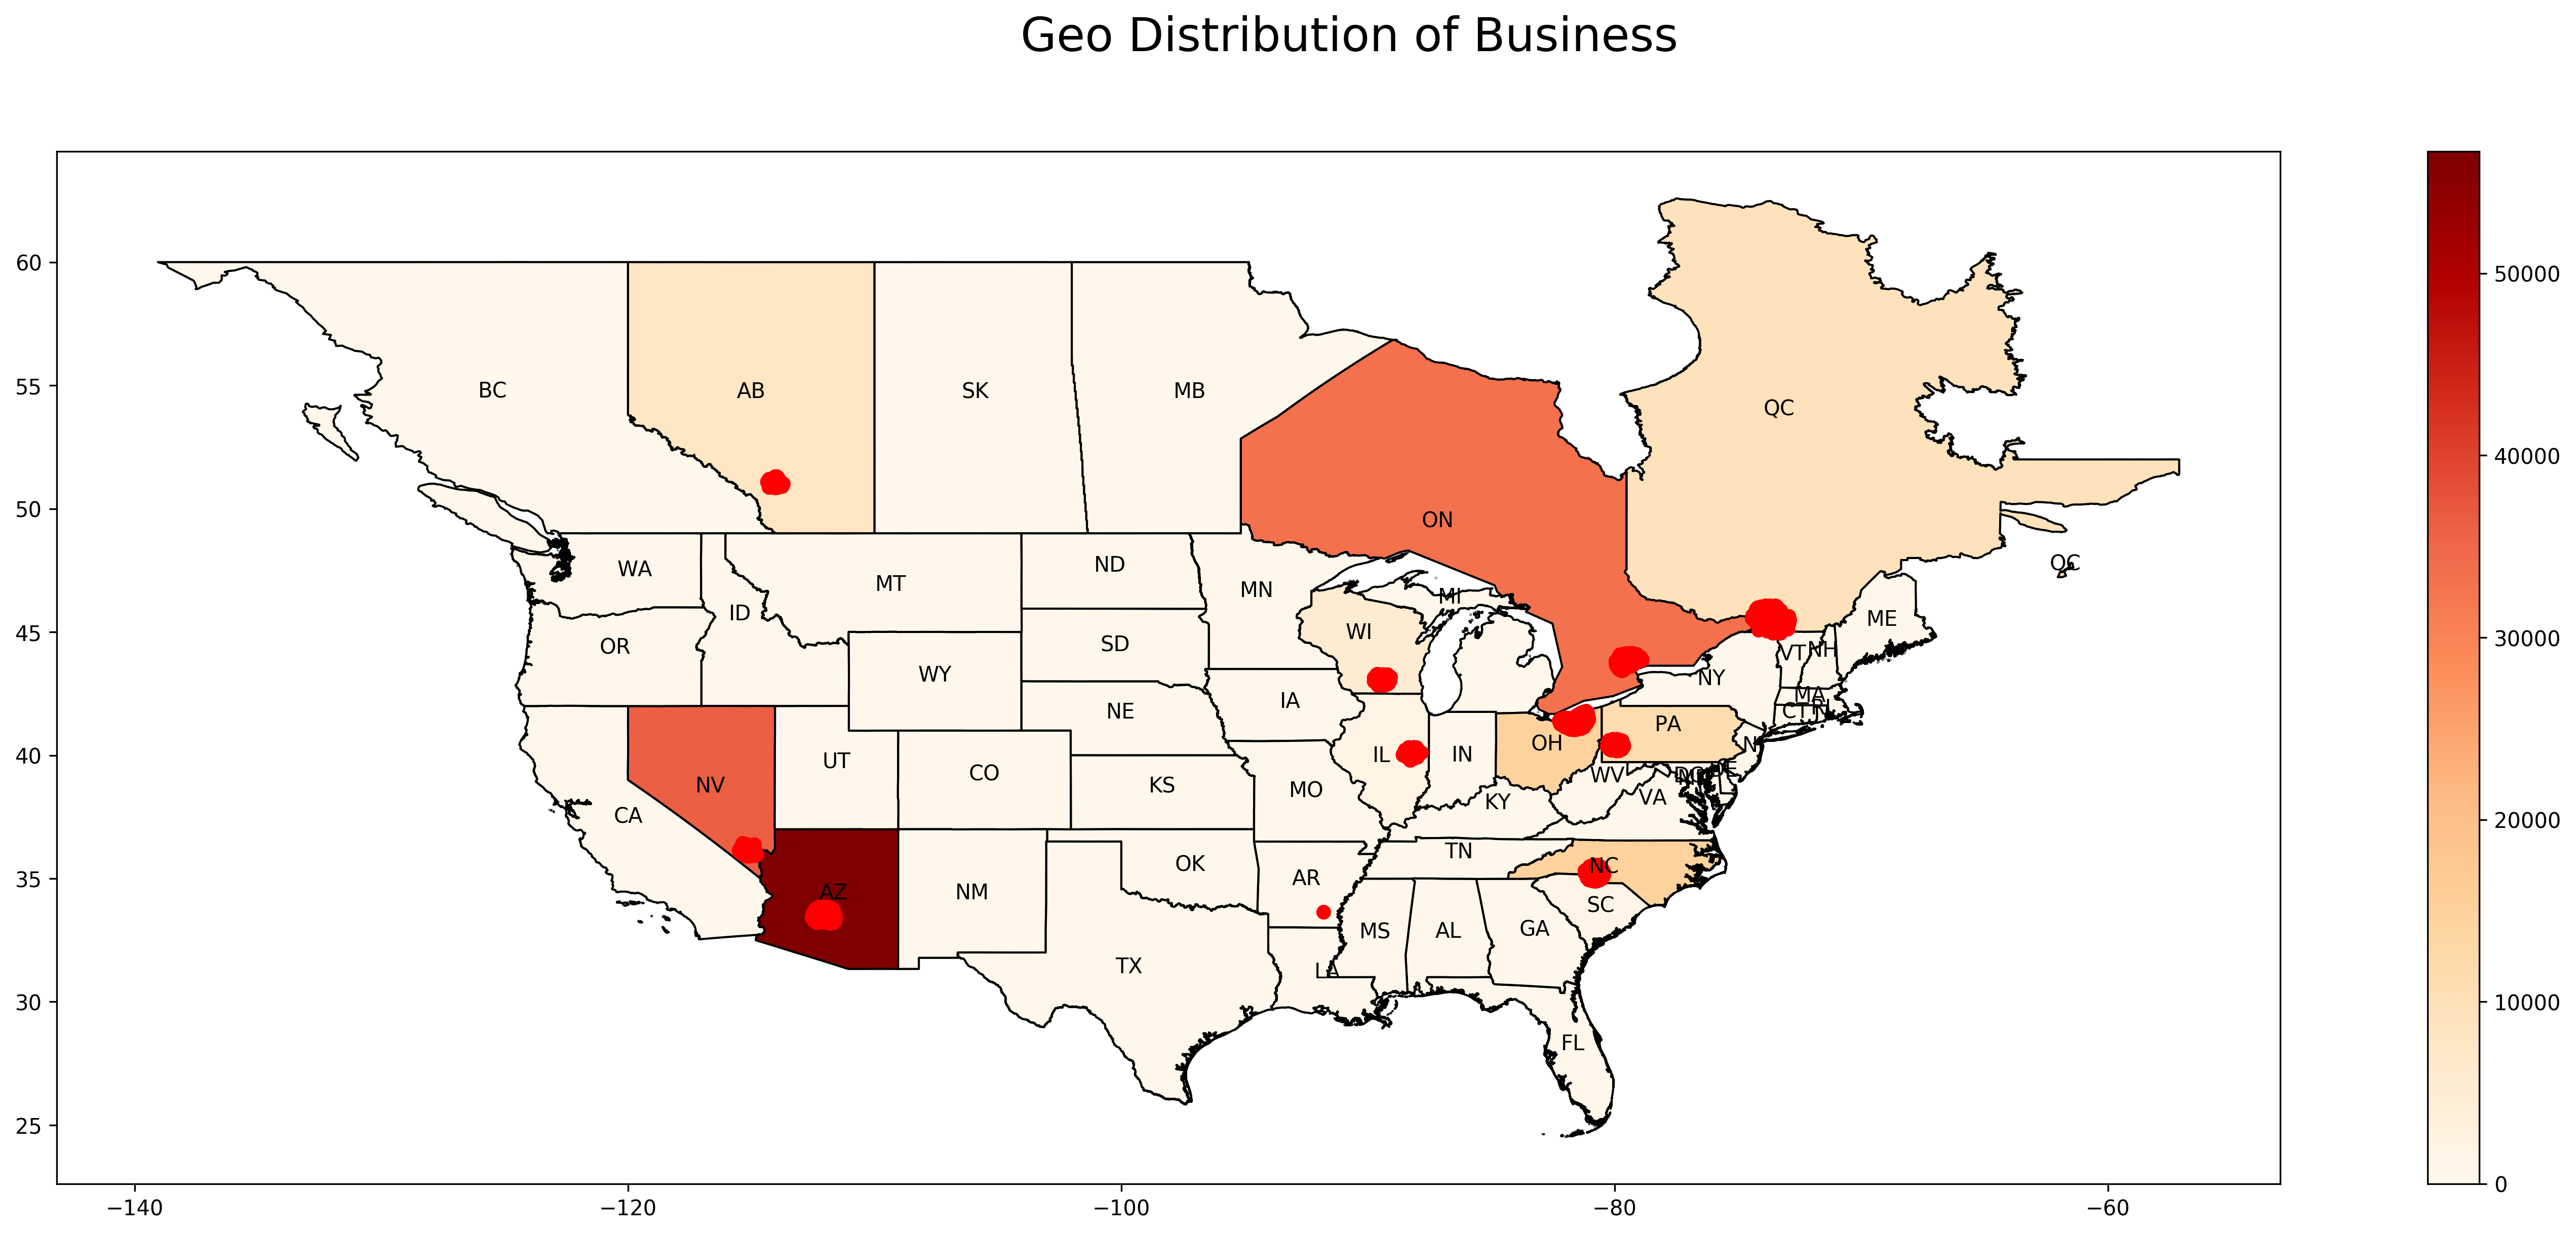
\includegraphics[width=1.0\textwidth]{../05_dataMining/distributionBusinessGeo.png}
\end{center}
\end{figure}
We can get from the plot where are the 10 metropolitan areas that the data came from. Most of them are from the USA and Canada, a small amount of reviews from Alaska and the UK are not shown on this plot.

\subsubsection{Distribution of Registered Users Over Time}
\begin{figure}[H]
\begin{center}
    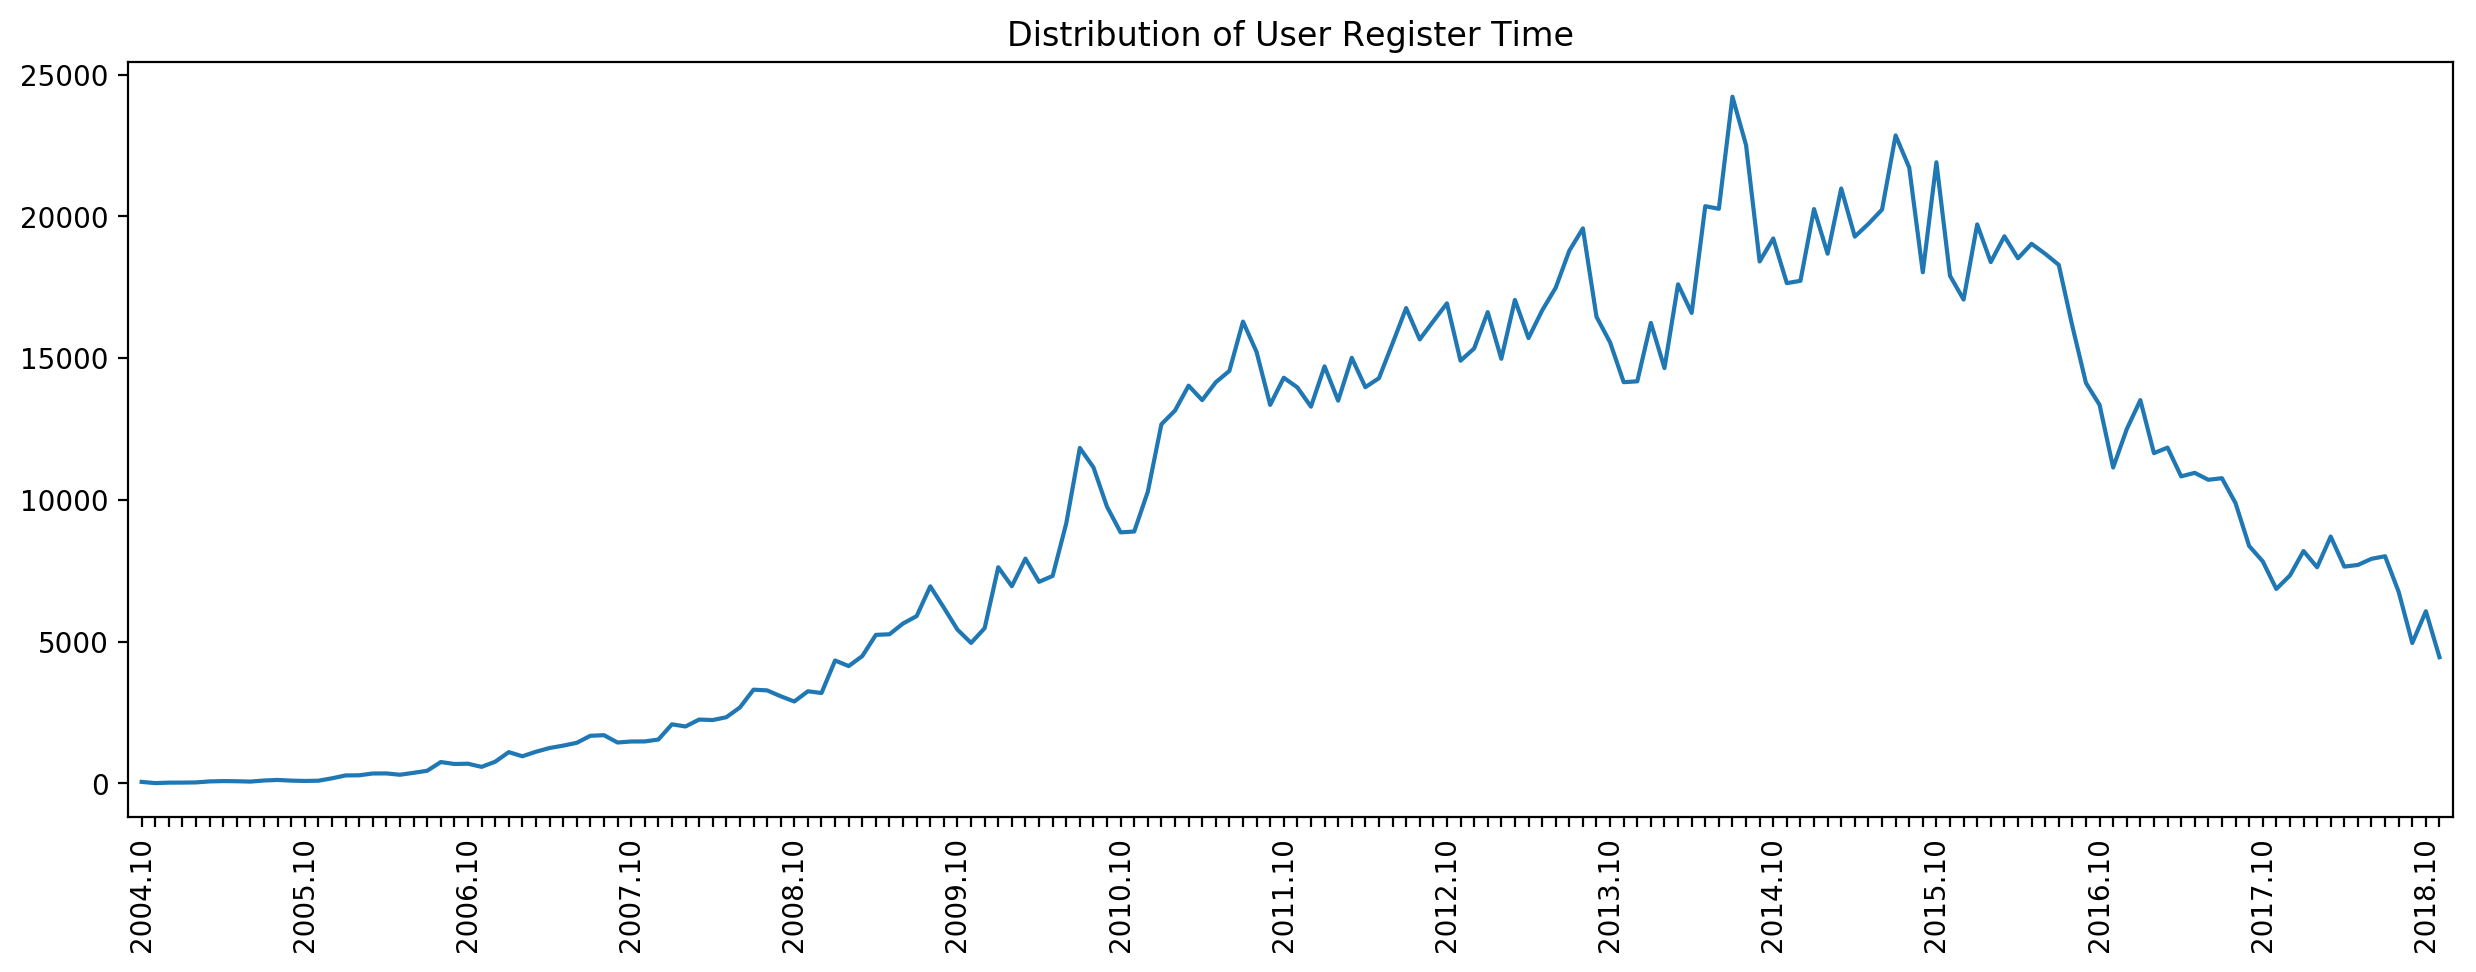
\includegraphics[width=1.0\textwidth]{../05_dataMining/distributionUserRegisterTime.png}
\end{center}
\end{figure}
The peak of the user register time is from 2014 to 2016. The amount of new user started to decrease since 2016. 

\subsubsection{User Satisfaction VS User Register Time}
\begin{figure}[H]
\begin{center}
    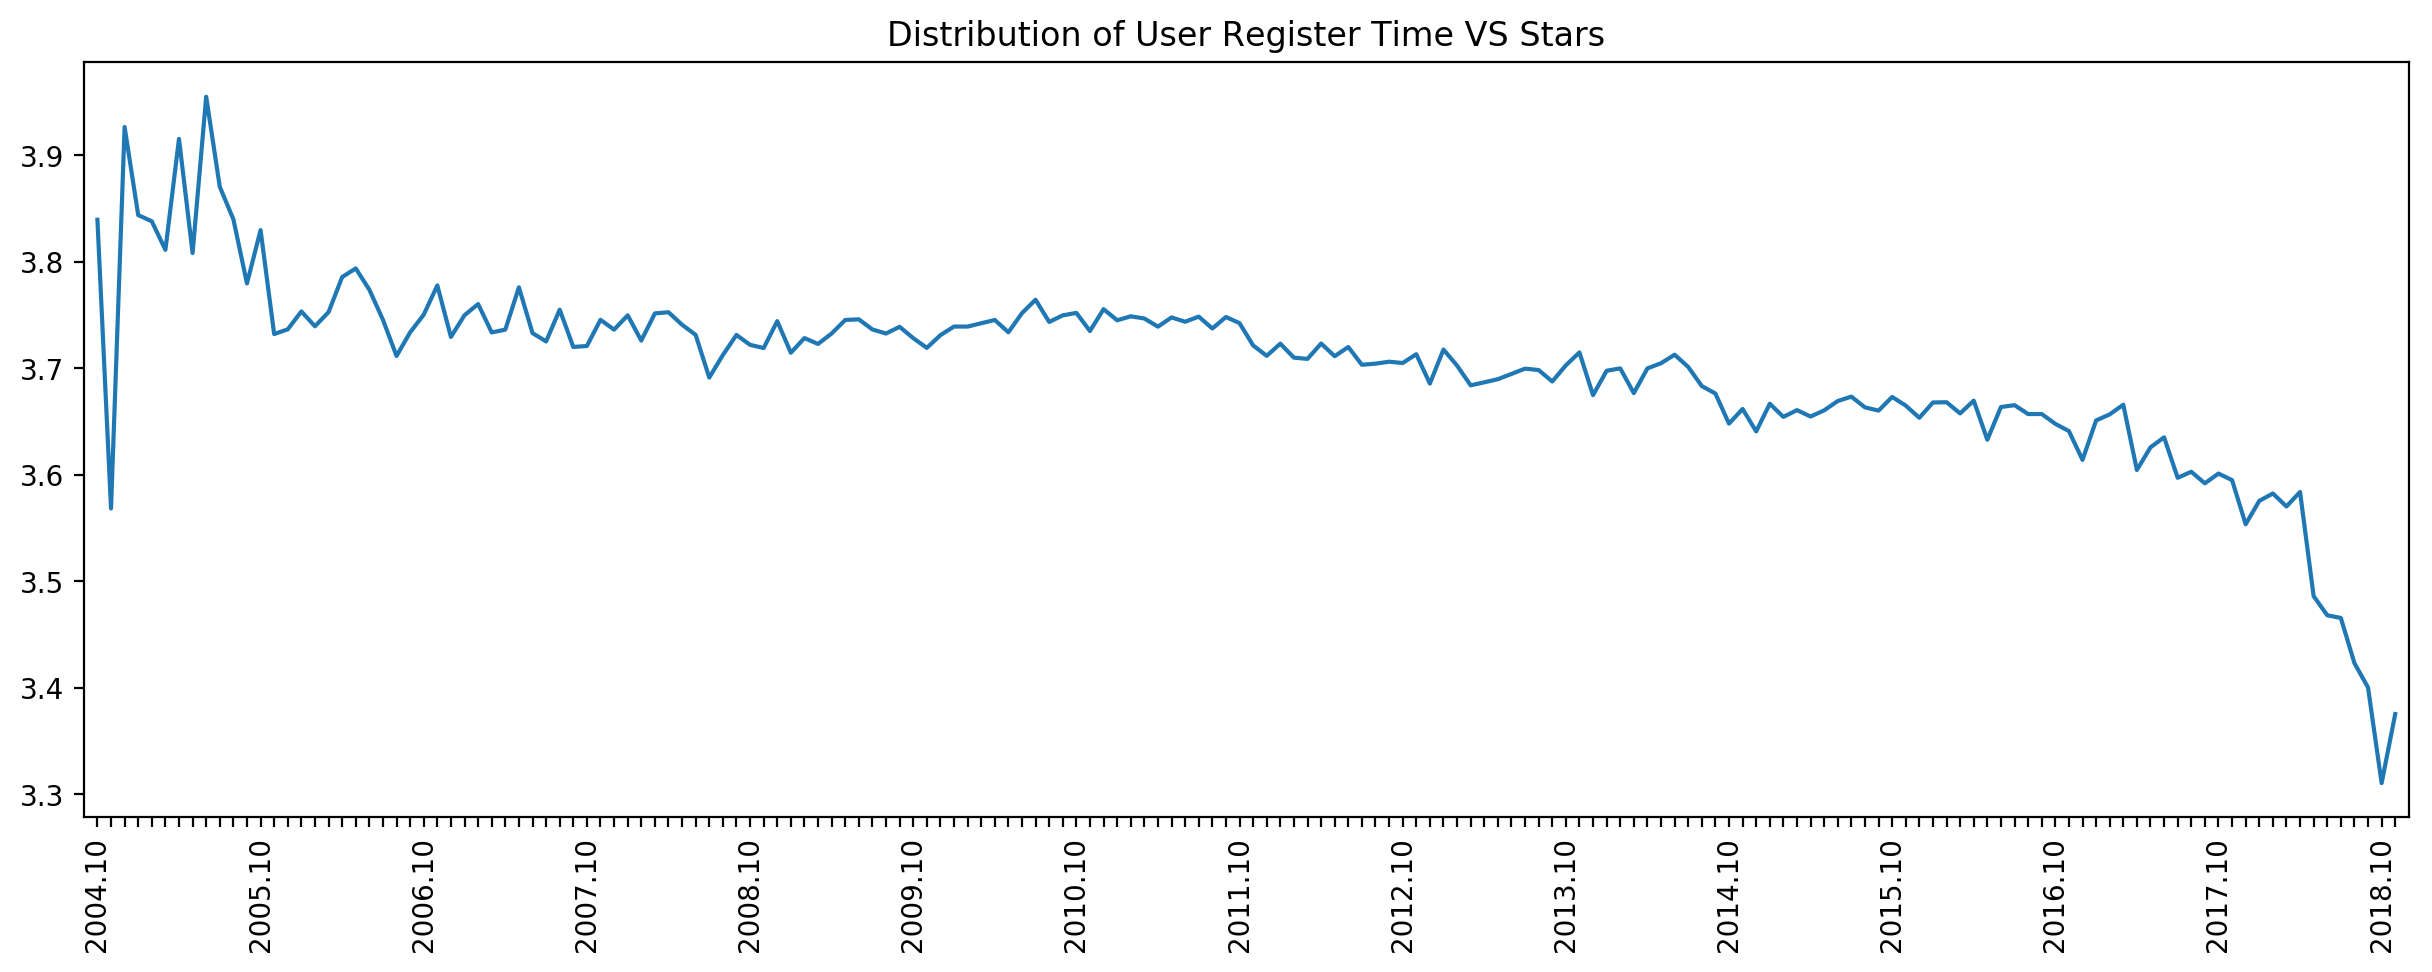
\includegraphics[width=1.0\textwidth]{../05_dataMining/distributionUserRegisterTimeStars.png}
\end{center}
\end{figure}
The average score a user will give gradually decrease with a user's register time, which means the newer a user is, the more likely he/she will give a lower score to a business, which means the users are more and more difficult to satisfy over time.

\subsubsection{Comparison Between Normal Users and Elite Users}
\begin{figure}[H]
\begin{center}
    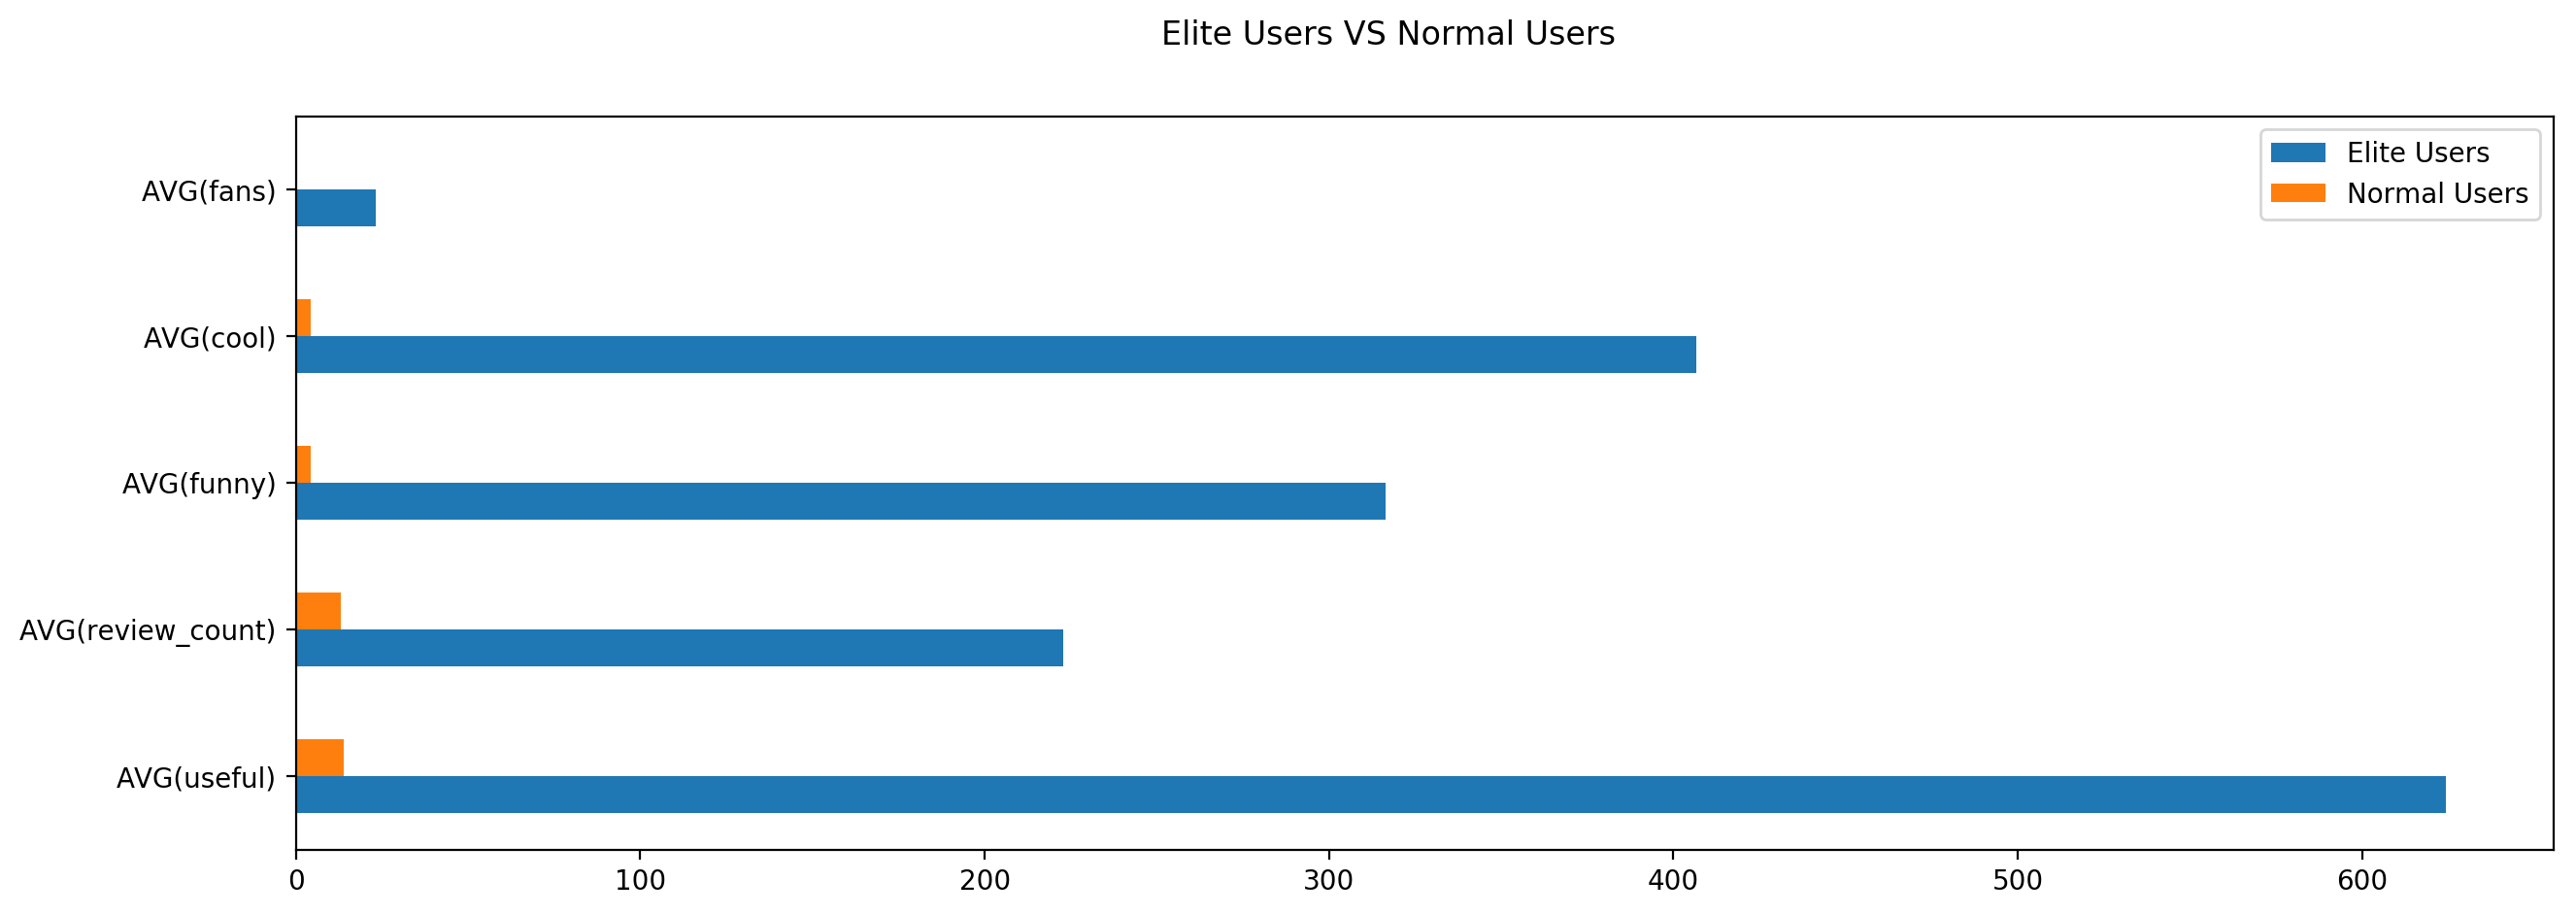
\includegraphics[width=1.0\textwidth]{../05_dataMining/eliteVSNormalUsers.png}
\end{center}
\end{figure}
On average, an elite user has more than 600 useful count, 200 review count, 300 funny count, 400 cool count and 20 fans, which are dozens to hundreds of times greater than those of the normal users. It is indeed not easy to become an elite user.

\subsubsection{Distribution of the User Review Number}
\begin{figure}[H]
\begin{center}
    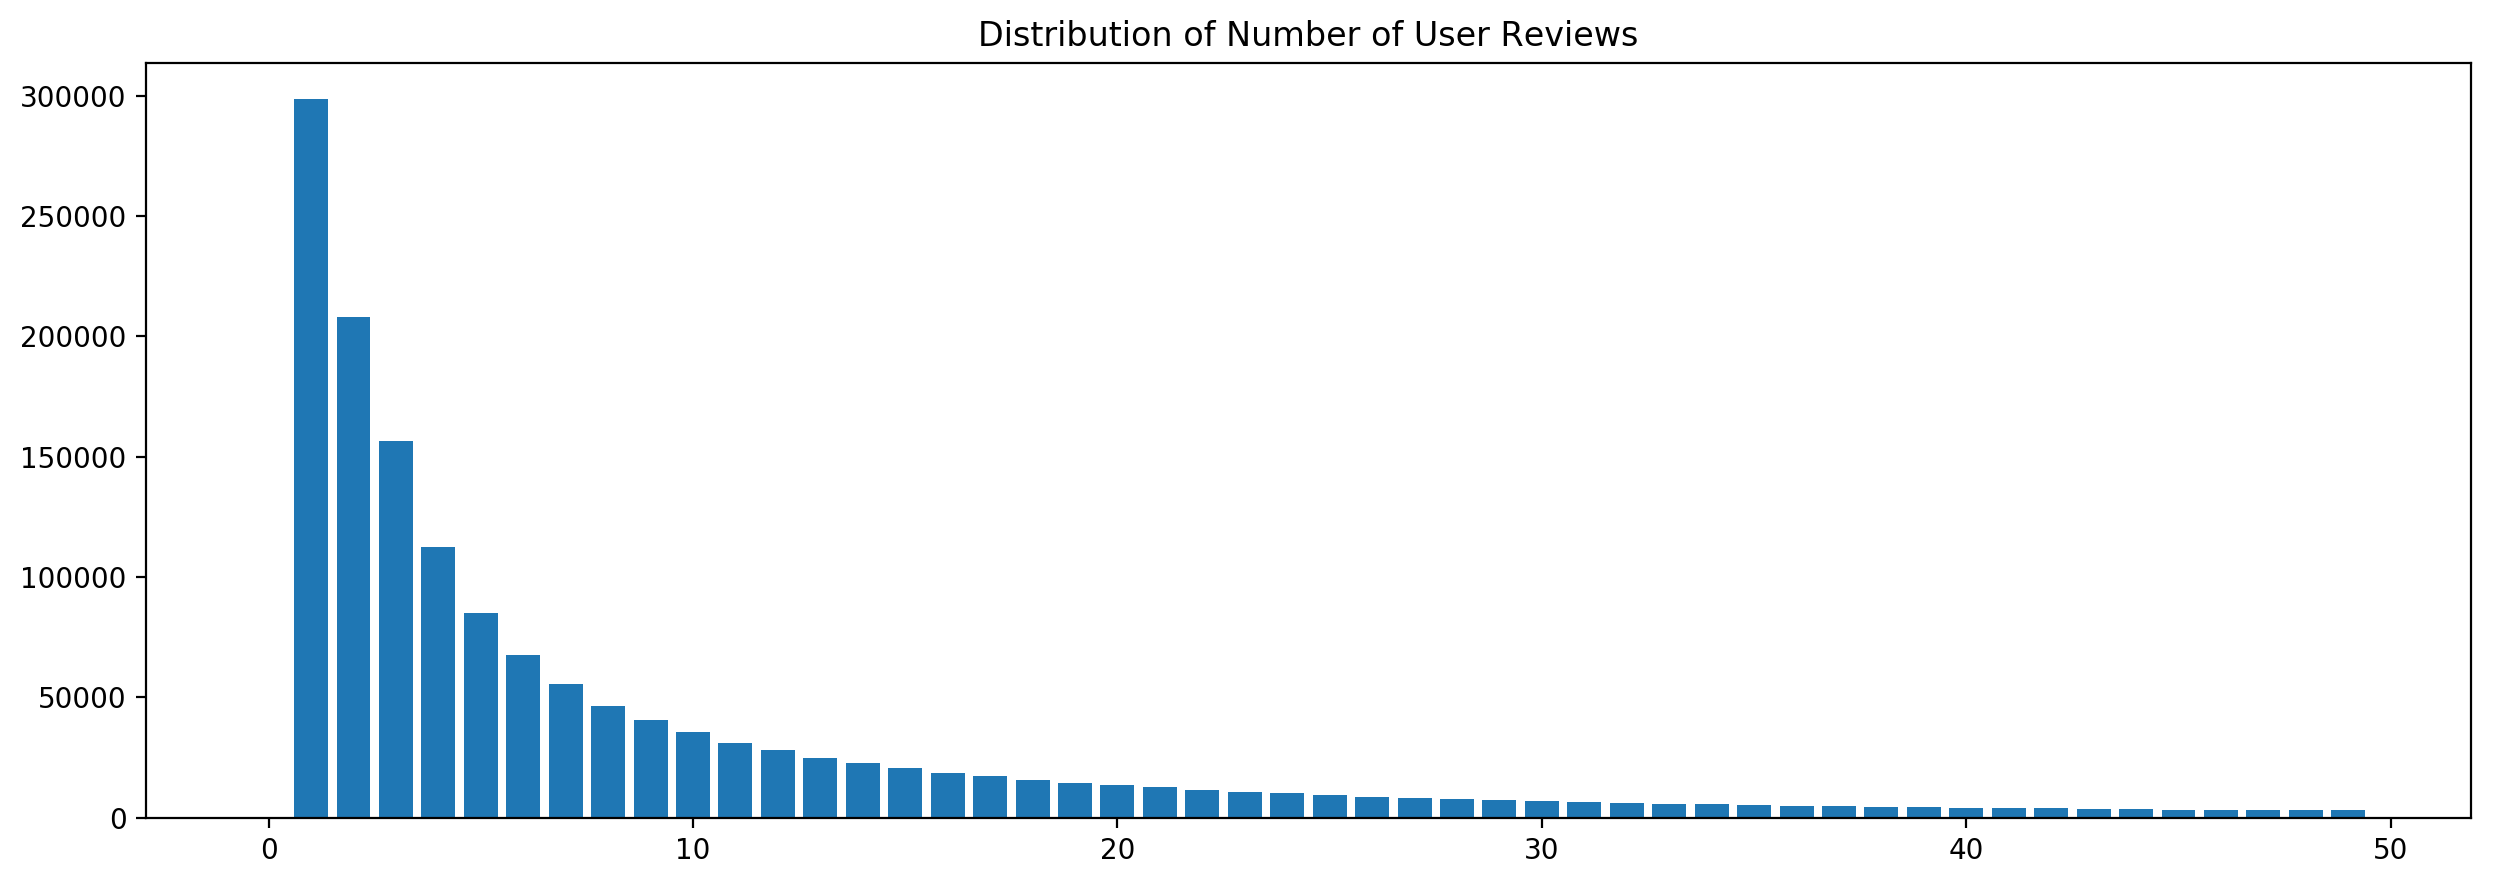
\includegraphics[width=1.0\textwidth]{../05_dataMining/distributionNumUserReviews.png}
\end{center}
\end{figure}
More than 90 percent of users have less or equal than 10 reviews.

\subsubsection{User Checkin Time for Each Day in a Week}
\begin{figure}[H]
\begin{center}
    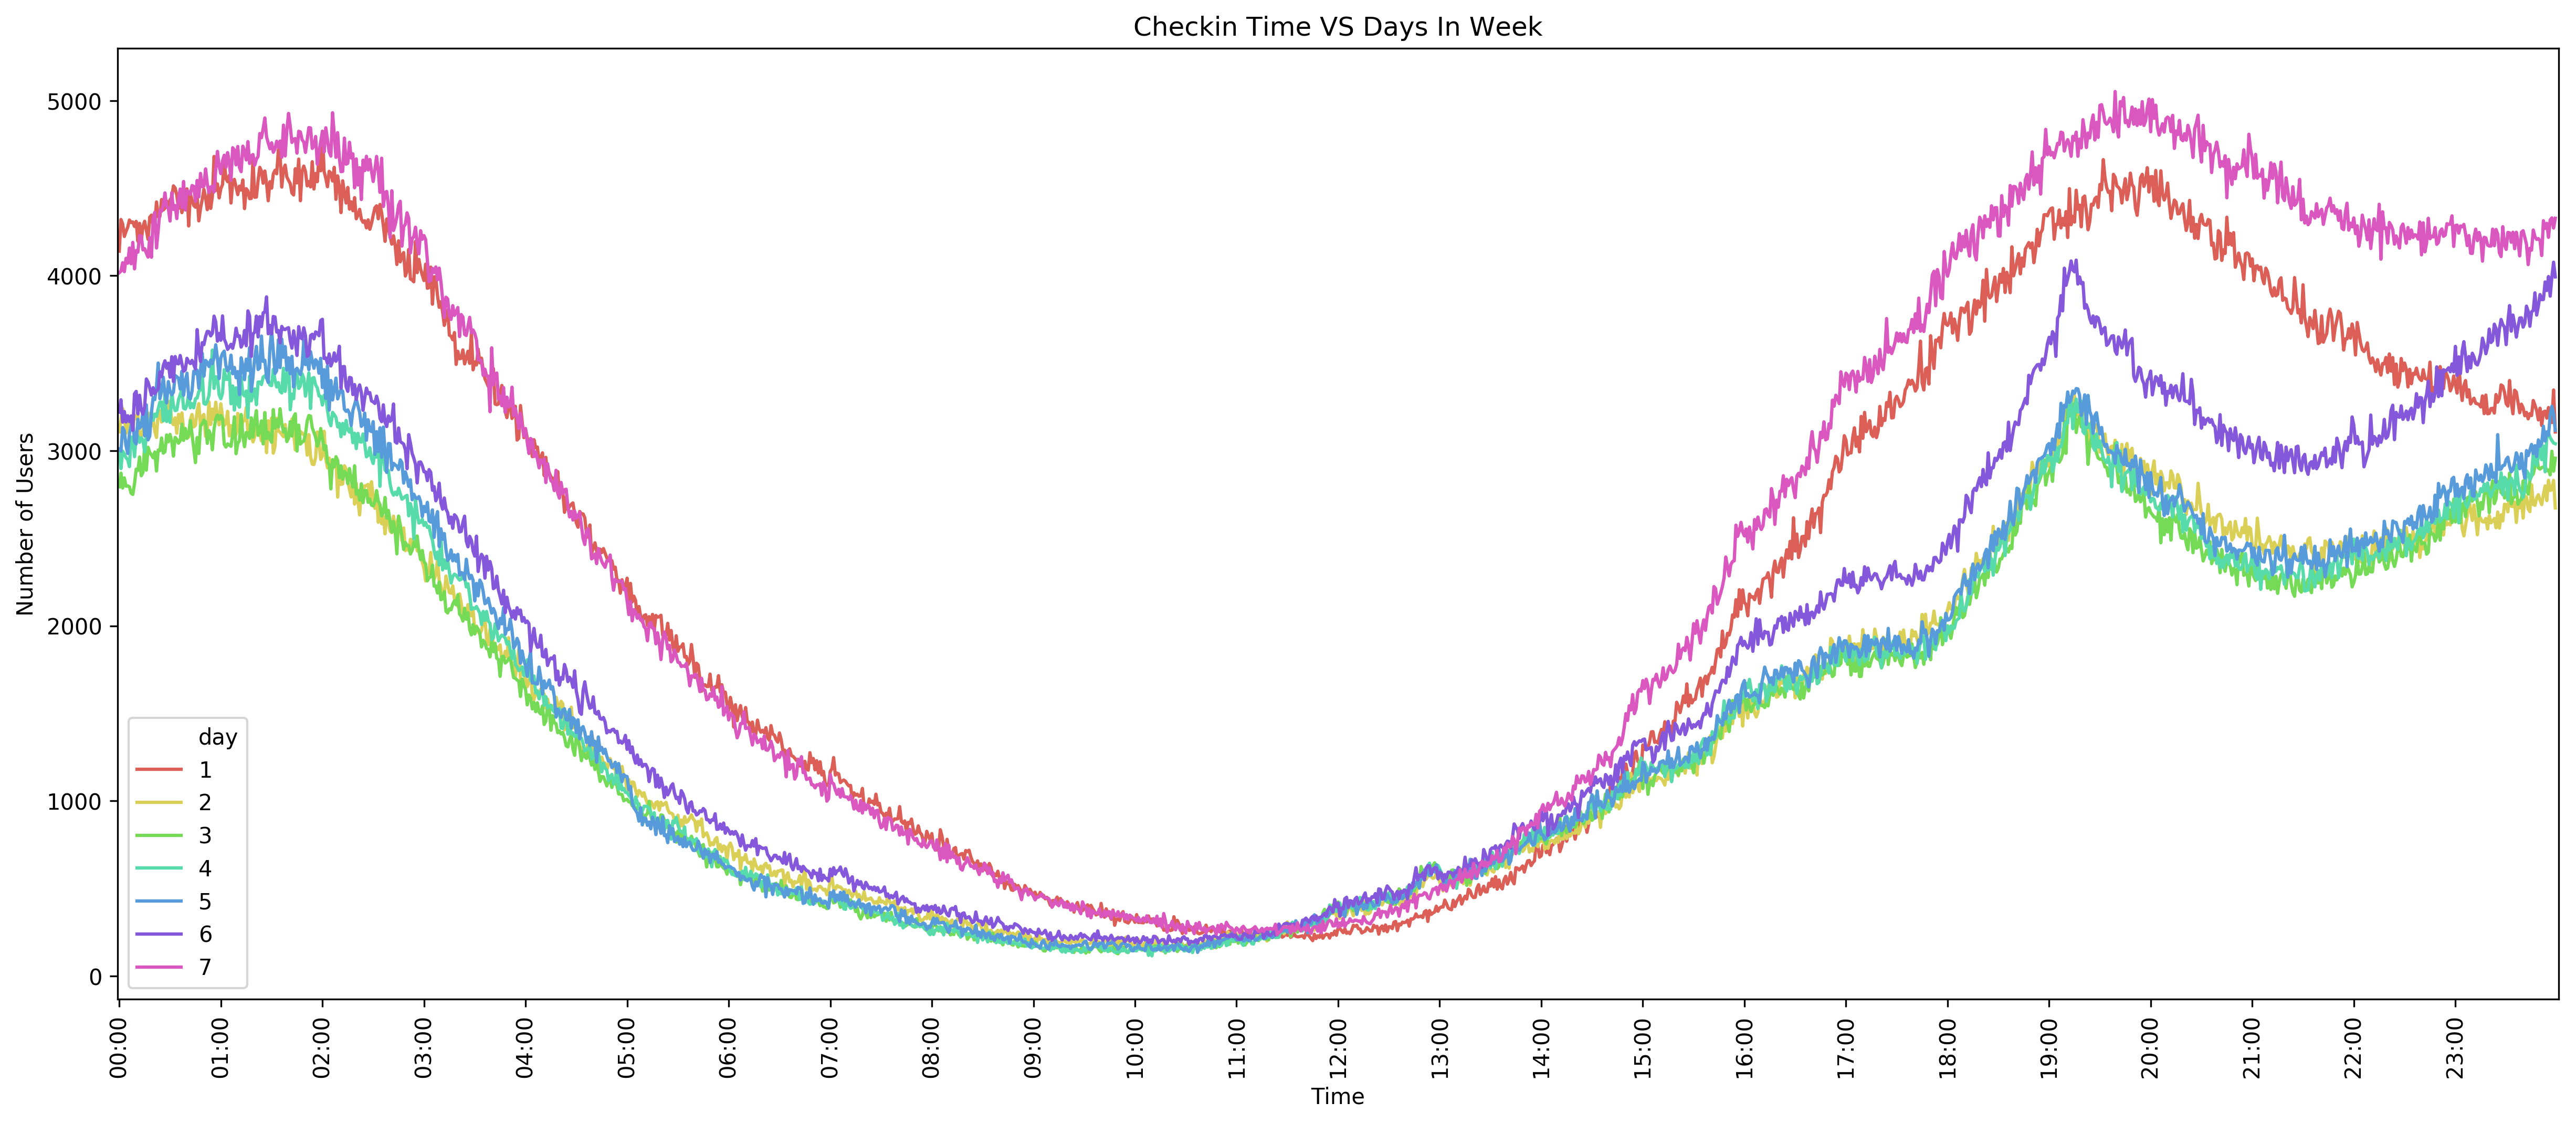
\includegraphics[width=1.0\textwidth]{../05_dataMining/checkinTimeVSDay.png}
\end{center}
\end{figure}
Users are more likely to check in on a business from 7PM to 2 AM, which is reasonable because people were off work and finished their dinner around that time. And there are most checkins on Sunday and Monday, which is probably because people went to that restaurant or store on Saturday and Sunday, and one day later they wrote reviews about that business.

\subsubsection{Useful number VS Word Count in a Review}
\begin{figure}[H]
\begin{center}
    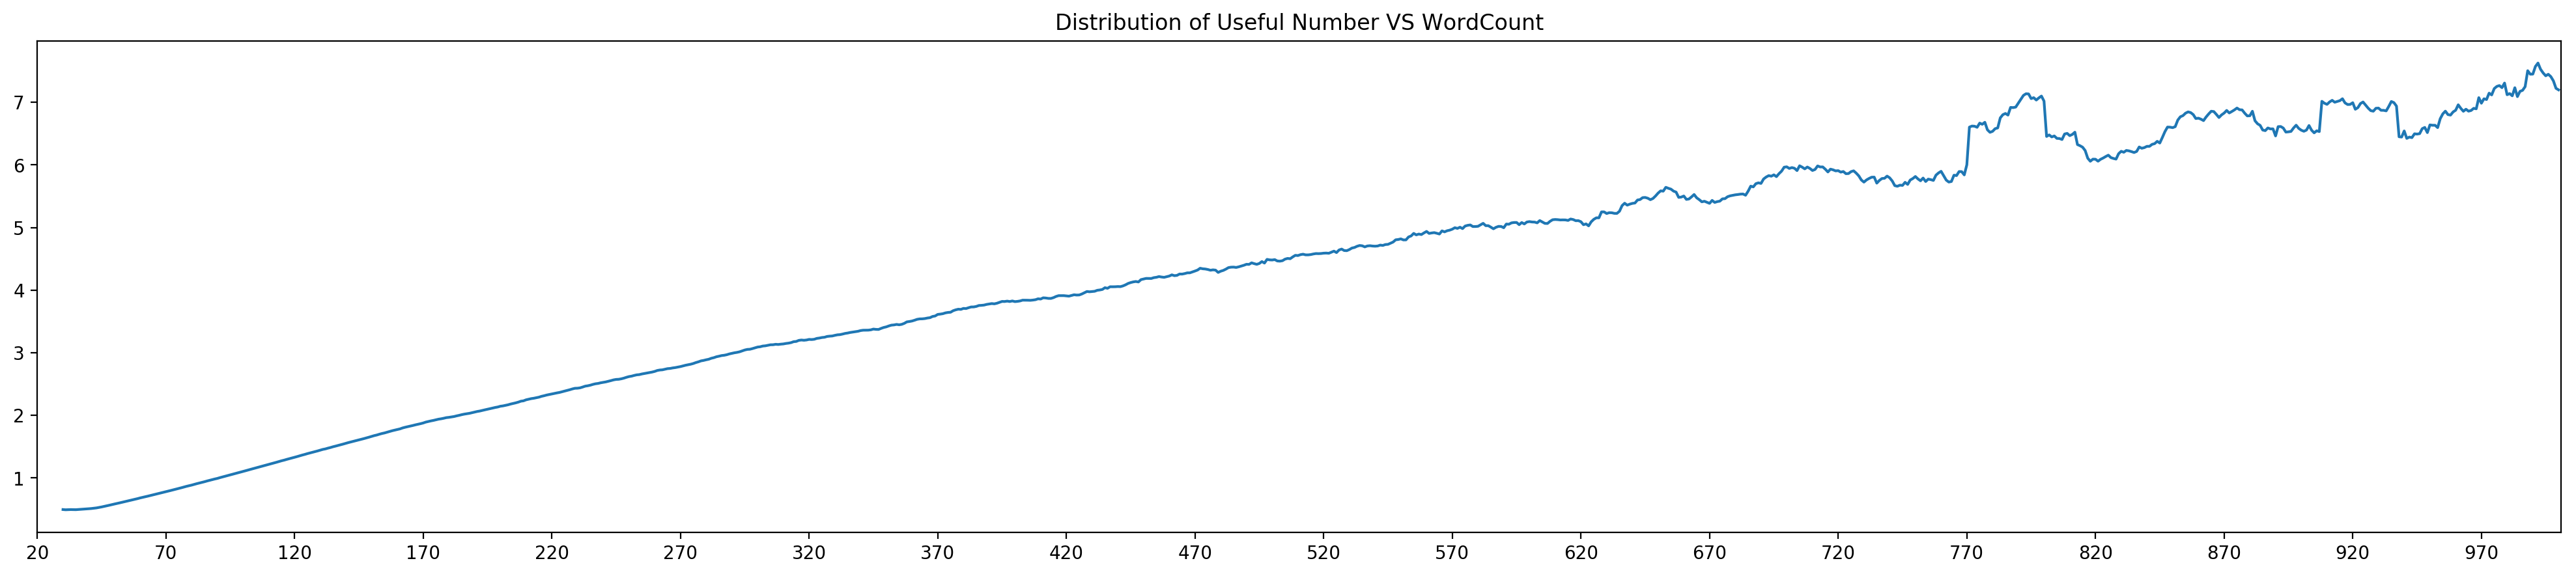
\includegraphics[width=1.0\textwidth]{../05_dataMining/distributionUsefulWordCount.png}
\end{center}
\end{figure}
The more words in a review, the more likely it is tagged as useful.
\subsection{Classification}
We perform classification on review stars(1.0 to 5.0) based on the content of a review. 125,000 reviews are selected for the classification, in which 80\% are used for training and 20\% are used for testing. We cannot preform classifiers on texts directly, so the texts are converted to a matrix of TF-IDF features using TfidfVectorizer in sklearn.
\subsubsection{Classification without PCA}
Apply Naive Bayes Classifier, Logistic Regression and Random Forest Classifier on the training data. (Timeout on other classifiers.) Then plot their confusion matrices using testing data.
\begin{figure}[H]
\captionsetup[subfigure]{labelformat=empty}
\centering
\subfloat[]{\includegraphics[width=0.33\textwidth]{"../05_dataMining/Naive Bayes Confusion Matrix"}}
\subfloat[]{\includegraphics[width=0.33\textwidth]{"../05_dataMining/Logistic Regression Confusion Matrix"}}
\subfloat[]{\includegraphics[width=0.33\textwidth]{"../05_dataMining/Random Forest Confusion Matrix"}}
\end{figure}
We can see that all of these three classifiers can classify the 1 and 5 stars reviews really well. But they tend to predict 4 and 3 stars and sometimes even 2 stars reviews as 5 stars reviews. And they also tend to predict 2 stars reviews as 1 star reviews. Overall, 2 stars reviews are the most difficult ones to predict, following by 3 stars and 4 stars because the words used in those reviews are really similar to each other and sometimes even a human cannot tell which class they should be in. If we specify that a review that greater or equal to 3 stars is good and otherwise is bad, and do a binary classification, the result will be much better.

We can get the most positively related words and the most negatively related words in the review from the trained logistic regression model. Those words play a decisive role in the classification. Their wordclouds with top 20 words are shown below:
\begin{figure}[H]
\captionsetup[subfigure]{labelformat=empty}
\centering
\subfloat[]{\includegraphics[width=0.5\textwidth]{"../05_dataMining/Logistic Regression Worst Words"}}
\subfloat[]{\includegraphics[width=0.5\textwidth]{"../05_dataMining/Logistic Regression Best Words"}}
\end{figure}

For random forest classifier, we cannot distinguish the "best" and the "worst" words, but we can still get the crucial words. The wordcloud with top 30 words are shown below:
\begin{figure}[H]
\begin{center}
    \includegraphics[width=0.5\textwidth]{"../05_dataMining/Random Forest Top Words"}
\end{center}
\end{figure}
\subsubsection{Classification with PCA}
The dimension of the raw data is rather high, making it impossible to run some algorithms. We first run standard scalar on the data, which is required by PCA. Then we draw the scree plot of PCA.
\begin{figure}[H]
\begin{center}
    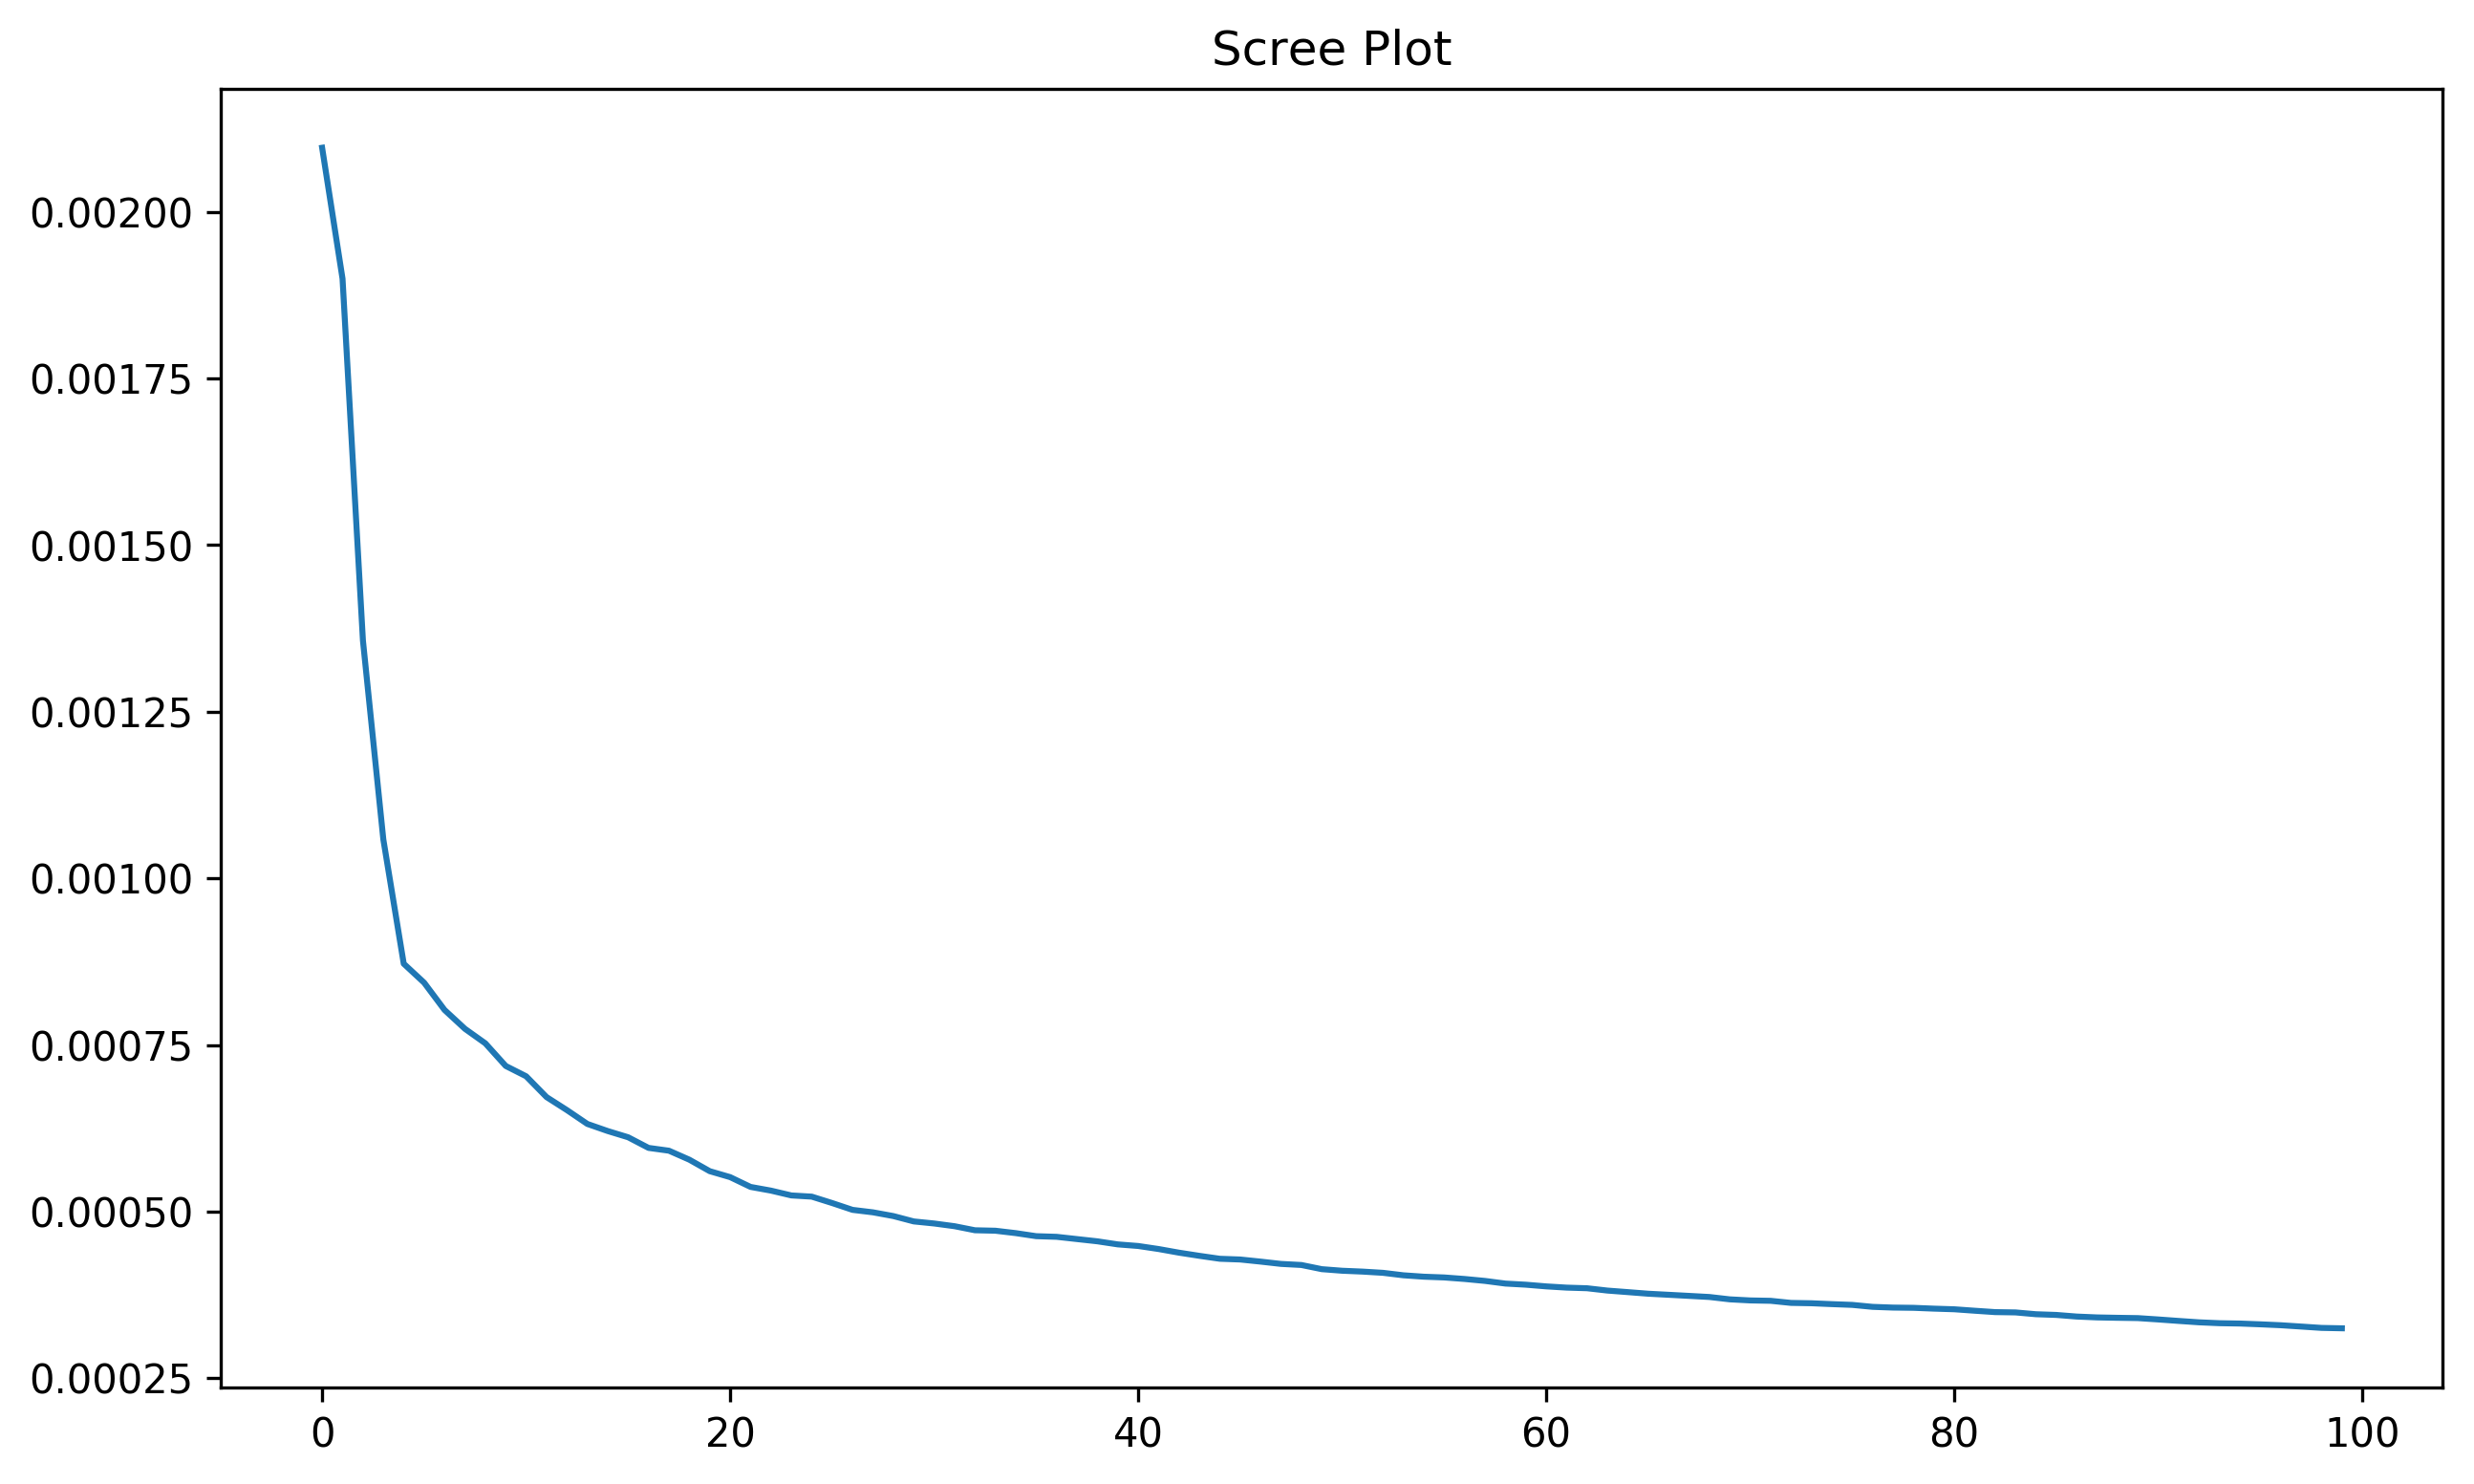
\includegraphics[width=0.6\textwidth]{../05_dataMining/ScreePlot.png}
\end{center}
\end{figure}
From the scree plot we know that each of the selected components explains a really small percentage of varince. Based on the plot, we use n\_components=50 to process our data.

Then, we apply logistic regression, random forest, adaboost, LDA, decision tree and KNN classifiers on it. (PCA makes some value negative, therefore we cannot use Naive Bayes classifier. Also, Naive Bayes based on applying Bayes' theorem with strong independence assumptions between the features, and preprocessing will seriously impact the result.) Their confusion matrices are as below:
\begin{figure}[H]
\captionsetup[subfigure]{labelformat=empty}
\centering
\subfloat[]{\includegraphics[width=0.33\textwidth]{"../05_dataMining/Logistic Regression(PCA) Confusion Matrix"}}
\subfloat[]{\includegraphics[width=0.33\textwidth]{"../05_dataMining/Random Forest(PCA) Confusion Matrix"}}
\subfloat[]{\includegraphics[width=0.33\textwidth]{"../05_dataMining/AdaBoost(PCA) Confusion Matrix"}}
\end{figure}
\vspace*{-1.5cm}
\begin{figure}[H]
\captionsetup[subfigure]{labelformat=empty}
\centering
\subfloat[]{\includegraphics[width=0.33\textwidth]{"../05_dataMining/LDA(PCA) Confusion Matrix"}}
\subfloat[]{\includegraphics[width=0.33\textwidth]{"../05_dataMining/Decision Tree(PCA) Confusion Matrix"}}
\subfloat[]{\includegraphics[width=0.33\textwidth]{"../05_dataMining/KNN(PCA) Confusion Matrix"}}
\end{figure}
Desision Tree classifier generates the worst result. It is merely better than random guess when predicting the 2, 3 and 4 stars revivews.

The performance of KNN and Adaboost is average. After PCA, the accuracy of both Logistic Regreesion and Random Forest decreases a bit. But Logistic regression is still the best method to split different reviews. And LDA is also a good method on this problem. 

However, most classifiers run under default parameters, with grid search to find better parameters and other preprocessing methods, the performance of these classifiers may be better.
\end{document}